% =====================================================================
%  DESARROLLO (versión integrada)
%  La estructura es la de main_objetivos: una sección por objetivo específico, sin números de
%  semana ni títulos literales de actividades, con cada campaña y video citado con el anexo A.
%  El contenido técnico que el recorte había quitado vuelve de capitulos/07-desarrollo.tex,
%  reubicado en el objetivo que le corresponde y sin fechas de bitácora.
% =====================================================================
\chapter{Desarrollo}
\label{cap:desarrollo}

Cada objetivo específico se cumplió con actividades de las fases que fijó la metodología del anteproyecto: el levantamiento de requisitos y el diseño conceptual responden al primero; el desarrollo progresivo, al segundo y al tercero; la integración, a los tres; y la validación, al cuarto. El registro de cada semana, el código, la matriz de requisitos con la prueba de cada uno, el protocolo experimental y el registro de cada misión están en el repositorio y en el sitio del proyecto (anexo B).

% =====================================================================
\section{Primer objetivo específico: arquitectura funcional}
\label{sec:oe1}

Modelar la arquitectura funcional exigía definir los requerimientos, los escenarios de operación con múltiples pisos, la estrategia de asignación de tareas y el esquema de comunicación entre agentes.

\subsection{Requerimientos del sistema}

El anteproyecto no enumeró los requisitos del sistema, aunque su metodología pedía verificar la implementación contra ellos. Por ello se identificaron a partir de los objetivos específicos, el alcance y el contrato de interfaces, y se formalizaron en una matriz de treinta y seis requisitos (tabla~\ref{tab:requisitos}), en la que cada uno cita su fuente y tiene una prueba que lo declara cumplido o no; un requisito sin prueba no entra en la matriz. Veintinueve describen funciones del sistema y siete son restricciones del alcance, como operar en interiores y en condiciones controladas o ejecutar la simulación en tiempo real. Al primer objetivo le corresponden diez, sobre arquitectura, coordinación y relevo; al segundo, seis, sobre la plataforma; al tercero, seis, sobre la interfaz; y al cuarto, siete, sobre las métricas, el registro de cada misión y las dos campañas. La confirmación de cambio de piso y la cancelación no estaban en el anteproyecto y se añadieron al ver el sistema en uso.

Del alcance salieron las restricciones que condicionan el diseño: el edificio no se interviene y ningún agente cambia de piso. El punto de transferencia es, por lo tanto, la escalera, y el chasis puede conservar la dirección tipo automóvil, ya que ningún agente tiene que entrar a un ascensor ni subir escalones, y la vuelta dentro del pasillo puede quedar a cargo de un planificador para automóviles.

\begin{table}[H]
  \centering\footnotesize\setstretch{1.0}
  \caption{Matriz de los treinta y seis requisitos del sistema, por objetivo específico, con la prueba que verifica cada uno.}
  \label{tab:requisitos}
  \begin{tabular}{@{}c>{\raggedright\arraybackslash}p{0.42\textwidth}>{\raggedright\arraybackslash}p{0.47\textwidth}@{}}
    \toprule
    \textbf{N.\textsuperscript{o}} & \textbf{Requisito} & \textbf{Prueba que lo verifica} \\ \midrule
    \multicolumn{3}{@{}l}{\textit{Primer objetivo específico: arquitectura funcional}} \\
    1 & Dos agentes, uno por piso & Dos pilas de navegación, una por agente \\
    2 & Cada agente se direcciona por separado & Una orden a un agente no altera al otro \\
    3 & Órdenes solo con la acción de navegación & Nadie fuera de cada agente publica velocidades \\
    4 & Catálogo de puntos de interés con piso y pose & El coordinador publica el catálogo completo \\
    5 & Misión asignada al agente del piso de origen & La solicitud activa solo al agente de ese piso \\
    6 & Mismo piso: un agente y ningún relevo & Misión sin relevos, con el segundo agente libre \\
    7 & Pisos distintos: protocolo de relevo & Dos tramos y transferencia, con un relevo \\
    8 & Cada agente publica su estado a 2~Hz & Frecuencia medida y cambio de estado en la misión \\
    9 & Entorno de dos pisos con punto de transición & El mundo carga los dos pisos y se navega el superior \\
    10 & Comunicación entre agentes por el coordinador & Ningún agente se suscribe a tópicos del otro \\ \addlinespace
    \multicolumn{3}{@{}l}{\textit{Segundo objetivo específico: plataforma robótica}} \\
    11 & Locomoción con cinemática Ackermann & Recorrido medido contra la odometría \\
    12 & Láser utilizable para localización y evasión & Frecuencia nominal y obstáculos en el mapa de costos \\
    13 & Cada agente publica su odometría & Lectura antes y después de un desplazamiento conocido \\
    14 & Mando desde ROS~2, sin la interfaz del fabricante & Una orden desde otra máquina de la red mueve al agente \\
    15 & Red entre agentes con latencia acotada & Mediana $\leq$ 100~ms, percentil 95 $\leq$ 250~ms, sin pérdidas \\
    16 & Mismo código en simulación y en agentes físicos & Compila en las dos distribuciones y completa misiones \\ \addlinespace
    \multicolumn{3}{@{}l}{\textit{Tercer objetivo específico: interfaz móvil}} \\
    17 & Selección de origen y destino & La selección en listas del catálogo lanza una misión \\
    18 & Estado de la misión en texto legible & Texto del coordinador literal en cada etapa \\
    19 & La interfaz habla solo con el coordinador & El puente no expone ningún tópico de los agentes \\
    20 & Acceso desde el navegador de un teléfono & Carga y operación completa desde un teléfono \\
    21 & El segundo tramo espera la confirmación & Confirmar, confirmar tras el aviso y no confirmar \\
    22 & Cancelación y regreso a la escalera & Misión cancelada a mitad de tramo y una de control \\ \addlinespace
    \multicolumn{3}{@{}l}{\textit{Cuarto objetivo específico: evaluación experimental}} \\
    23 & Registro del tiempo de respuesta & La misión registra las marcas de los dos eventos \\
    24 & Registro del tiempo de asignación & Banco de pruebas con el reloj del sistema \\
    25 & Registro del éxito o fallo, con su motivo & Éxito y motivo quedan en el registro \\
    26 & Registro de la continuidad entre niveles & Ninguna etapa sin agente activo entre los dos tramos \\
    27 & Métricas obtenidas de un registro automático & Un archivo por misión, procesable sin intervención \\
    28 & Campaña en simulación con 30 repeticiones & Treinta registros válidos \\
    29 & Demostración física con 5 a 10 repeticiones & Registros de las misiones con los agentes físicos \\ \addlinespace
    \multicolumn{3}{@{}l}{\textit{Restricciones del alcance}} \\
    30 & Ningún agente cambia de piso & Altura de cada agente constante durante la misión \\
    31 & Sin manipular objetos ni intervenir el edificio & Por diseño: el agente solo tiene tracción y dirección \\
    32 & Interiores y condiciones controladas & En la campaña, solo los dos autores en el pasillo \\
    33 & Plataforma de bajo costo & AWS DeepRacer en lugar de DonkeyCar \\
    34 & Trayectorias aptas para dirección Ackermann & Radio mínimo y sin giro sobre el propio eje \\
    35 & Simulación a tiempo real & Factor de tiempo real de 0,99 o más \\
    36 & Operación en un entorno conocido y mapeado & El mapa es un insumo de la misión \\ \bottomrule
  \end{tabular}
\end{table}

\subsection{Escenarios de operación con múltiples pisos}
\label{sec:entornos}

Los escenarios se definieron en dos edificios de la sede principal de la Universidad Santo Tomás, Gregorio y Catalayud, con dos pisos en cada uno (tabla~\ref{tab:entornos}). Los pisos 2 y 3 del edificio Gregorio fueron el entorno de la simulación y de la primera prueba de navegación con un agente físico, y los pisos 3 y 4 del edificio Catalayud, el de las pruebas de verificación y la campaña con los agentes físicos.

\begin{table}[H]
  \centering\footnotesize\setstretch{1.0}
  \caption{Pisos en los que se probó el sistema, con su uso, su planta y sus puntos de interés.}
  \label{tab:entornos}
  \begin{tabular}{@{}>{\raggedright\arraybackslash}p{0.12\textwidth}>{\raggedright\arraybackslash}p{0.28\textwidth}>{\raggedright\arraybackslash}p{0.23\textwidth}>{\raggedright\arraybackslash}p{0.29\textwidth}@{}}
    \toprule
    \textbf{Piso} & \textbf{Uso} & \textbf{Planta} & \textbf{Puntos de interés} \\ \midrule
    Gregorio, piso 2 & Simulación; campaña de treinta misiones & Pasillo con un hall en un extremo; 41,0~m de extensión en su mapa & 15: doce salones ETM, almacén ETM, «Representación» y escalera \\ \addlinespace
    Gregorio, piso 3 & Simulación; campaña de treinta misiones; prueba de navegación con un agente físico & Pasillo con un hall al oeste; 46,9~m de extensión en su mapa & 16: dos laboratorios de sistemas, once aulas, sala de docentes, rama IEEE y escalera \\ \addlinespace
    Catalayud, piso 3 & Pruebas de verificación y campaña con los agentes físicos; comprobación en simulación & Pasillo de norte a sur, de 25,3 a 25,5~m de largo y de 2,35 a 2,45~m de ancho & 5: salones 301, 302 y 303, ascensor y escalera, a 22,1~m del extremo norte \\ \addlinespace
    Catalayud, piso 4 & Los mismos que el piso 3 & Pasillo de norte a sur, de 25,5 a 25,6~m de largo y de 2,35 a 2,61~m de ancho & 5: salones 401, 402 y 403, ascensor y escalera, a 24,4~m del extremo norte \\ \bottomrule
  \end{tabular}
\end{table}

Cada piso del edificio Gregorio es un mundo de Gazebo con su mapa de navegación y sus puntos de interés en el catálogo, y en los dos la escalera queda en un hall al extremo del pasillo (figura~\ref{fig:mapas-gregorio}). El anexo A, en su video 2, muestra al agente teleoperado en el modelo del piso 2 de ese edificio.

\begin{figure}[H]
  \centering
  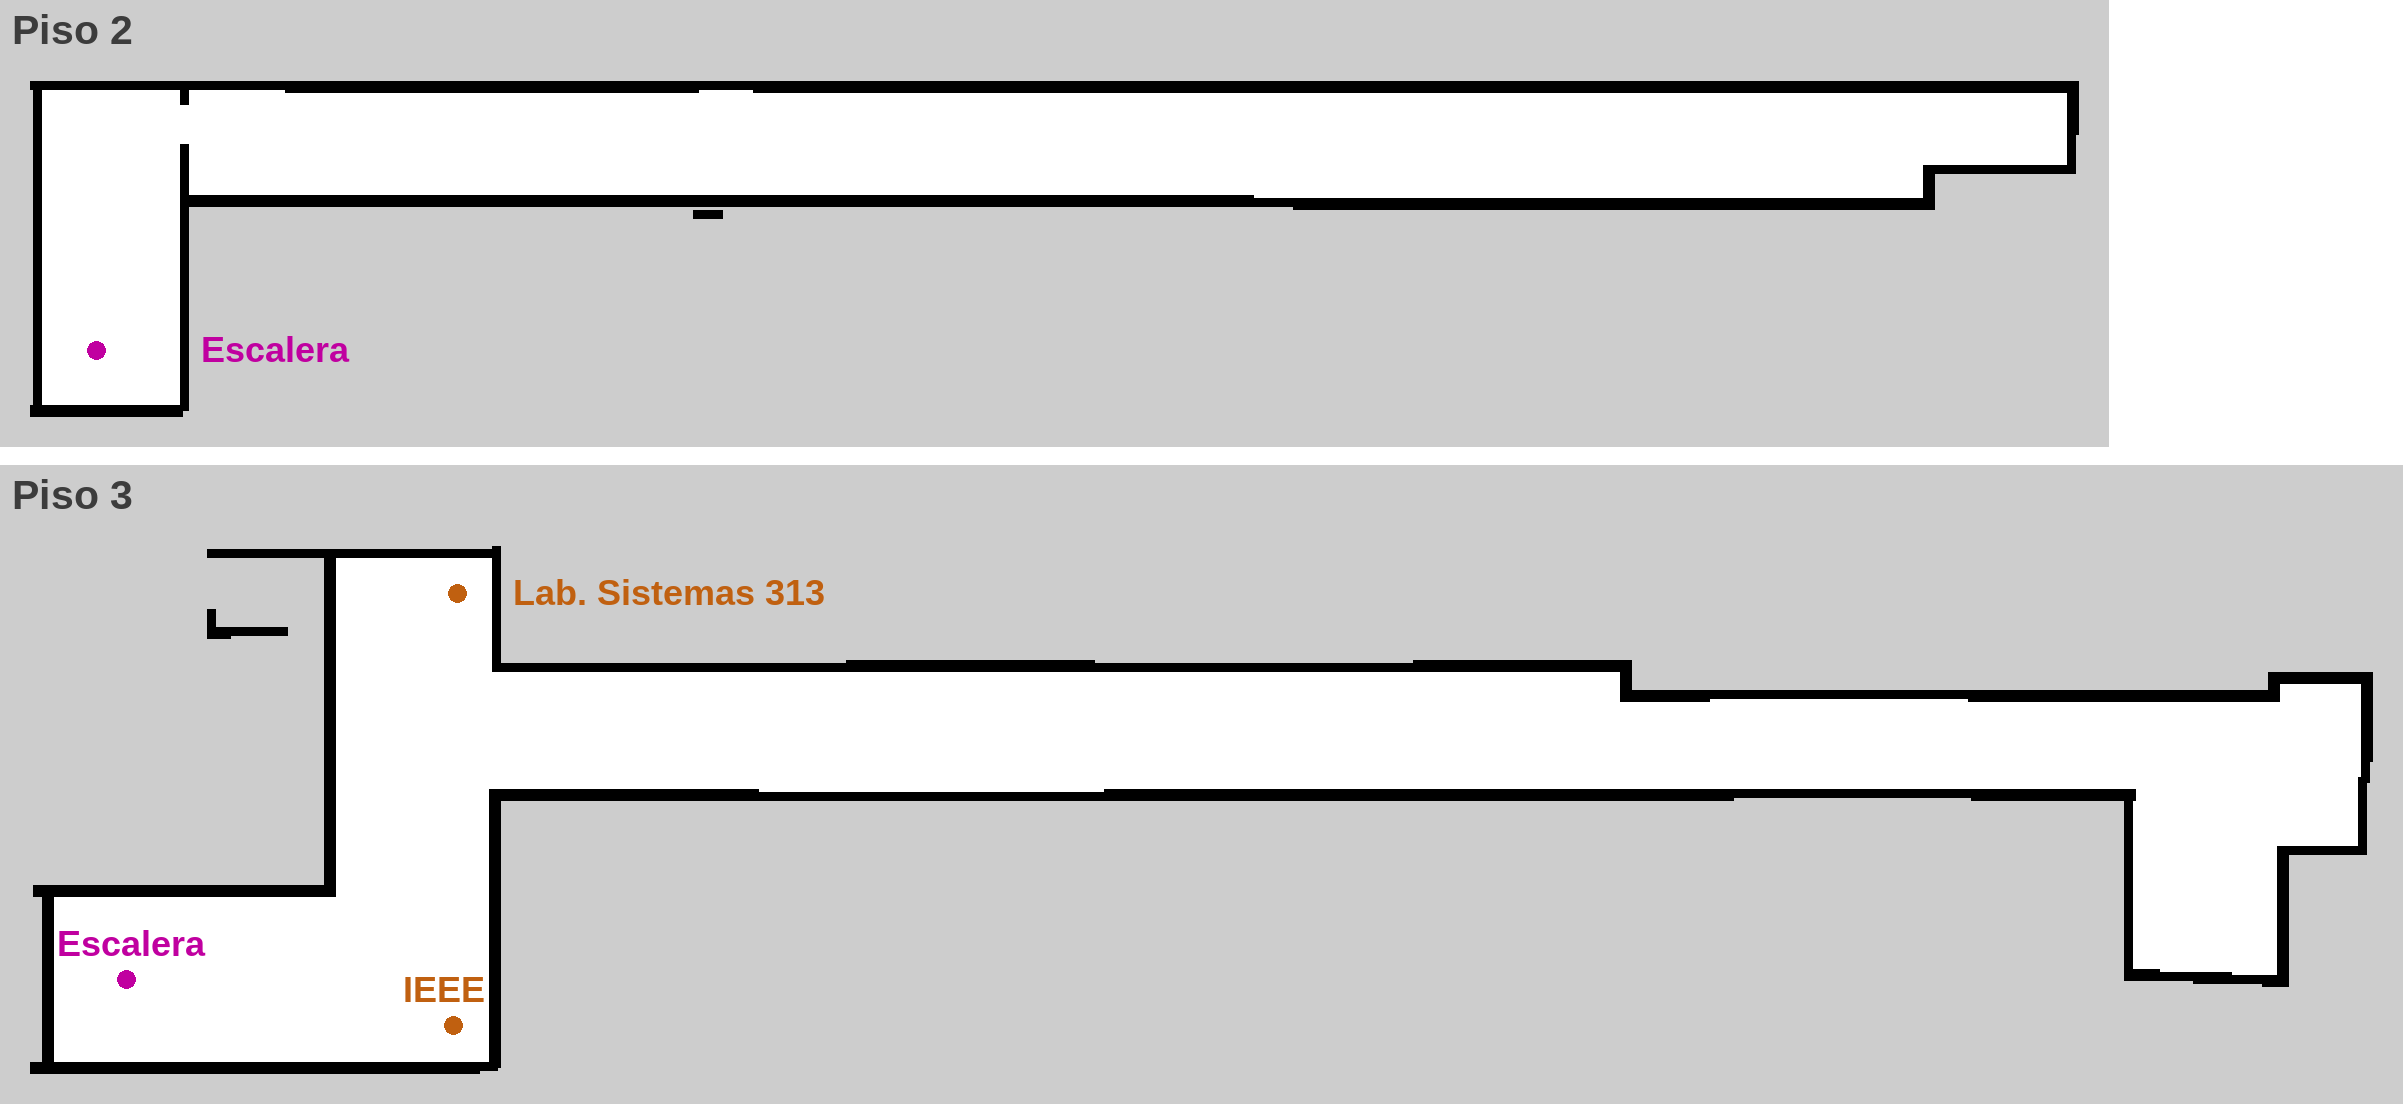
\includegraphics[width=0.8\textwidth]{imagenes/mapas_gregorio.png}
  \caption{Mapas de navegación de los pisos 2 (arriba) y 3 (abajo) del edificio Gregorio, calculados del modelo simulado, con el hall del piso 3 ya corregido.}
  \label{fig:mapas-gregorio}
\end{figure}

La prueba de navegación con un agente físico, en el hall del extremo oeste del piso 3 de Gregorio, no se superó: las dos llegadas medidas quedaron a 1,43 y 1,26~m del destino. La odometría no fue la única causa. El agente aún no tenía la unidad inercial, y la navegación no estaba ajustada para el agente físico, pues en esa misma sesión hubo que corregir una odometría invertida y subir el margen de llegada de Nav2 de 0,25 a 1,0~m. Además, el mapa cargado no correspondía al entorno real: la correspondencia entre el mundo simulado y el edificio se había dado por supuesta, y al verificarla resultó que el mundo daba el hall 0,84~m más ancho de lo que es, 4,24~m frente a 3,40~m, un 25~\% de error. Solo se comprobó esa pared, de modo que las demás medidas de ese modelo quedaron sin verificar.

Con el mapa sin corregir, la localización terminó a 1,17~m de lado de la posición medida con flexómetro, con una incertidumbre de hasta 3,44~m. Al corregirlo, el error de lado bajó a 0,15~m y la incertidumbre a 0,66~m, aunque a lo largo del hall la separación llegó a 2,62~m (figura~\ref{fig:hall}), con la odometría del láser registrando el 73~\% del avance. La campaña en simulación no depende de esa diferencia, ya que en ella el mundo y el mapa salen del mismo modelo. Con los agentes físicos se cambió de edificio, dado que en Gregorio el tránsito de personas dificultaba las pruebas, el modelo no correspondía a la planta real y, en sus pasillos rectos y uniformes, la odometría del láser no registraba el avance.

\begin{figure}[H]
  \centering
  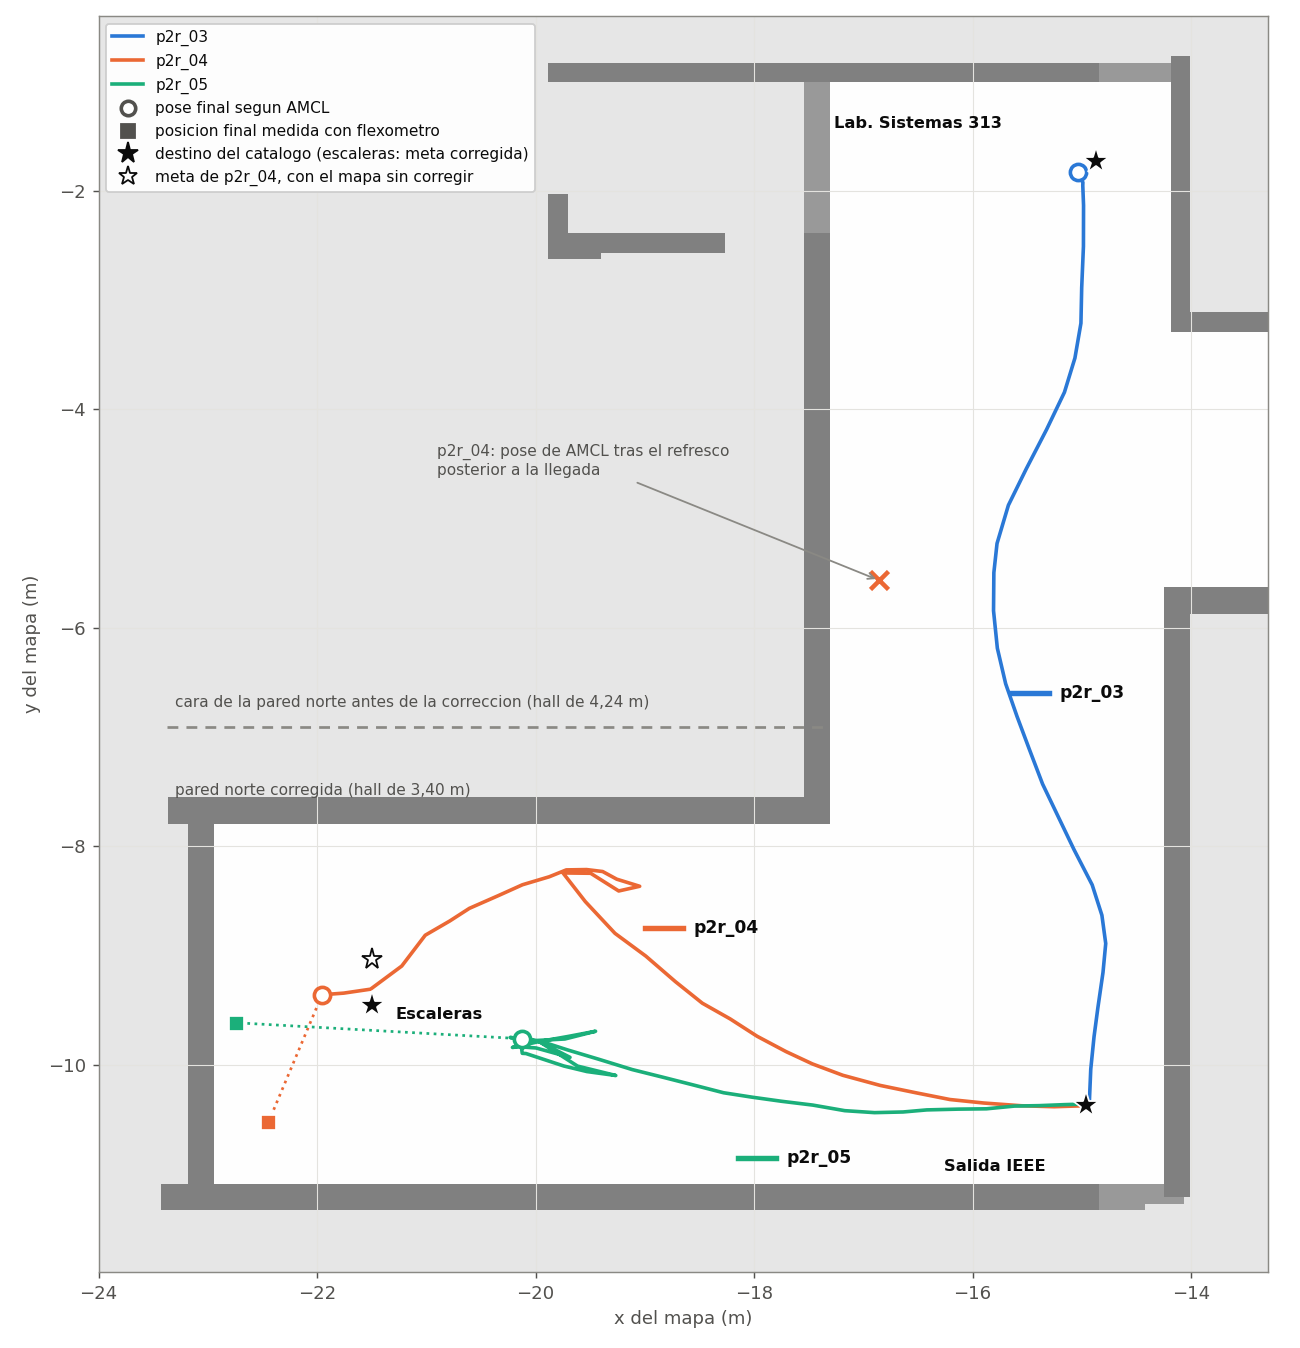
\includegraphics[width=0.5\textwidth]{imagenes/recorridos_hall_piso2.png}
  \caption{Tres recorridos de un agente en el hall del piso 3 del edificio Gregorio, sobre el mapa corregido: pose de la localización (círculo) y posición medida con flexómetro (cuadrado).}
  \label{fig:hall}
\end{figure}

El edificio Catalayud se eligió con un criterio que salió de esa medida: como el agente estima su avance comparando barridos sucesivos del láser, necesita estructura no uniforme dentro del alcance del sensor durante todo el recorrido. Sus pisos 3 y 4 la tienen, ya que entre las hornacinas de los salones, los casilleros, la papelera, el ascensor y la escalera suman ocho cambios de perfil en 25~m, uno cada tres metros. Cada piso es un pasillo recto, con los tres salones al este, en hornacinas de 0,99 y 1,01~m de fondo, y el ascensor y la escalera al oeste (figura~\ref{fig:mapas-catalayud}). La escalera es el punto de transferencia de cada piso, y los casilleros y la papelera se marcan en los mapas como referencia del levantamiento.

El mapeo con SLAM en los propios agentes no dio un mapa utilizable en ningún pasillo, por la misma falta de información de avance. En Catalayud se invirtió entonces el orden seguido en Gregorio: primero se midió y después se modeló. Los pisos 3 y 4 se levantaron con flexómetro, y de ese levantamiento se derivaron el mundo simulado, el mapa de navegación y el catálogo de destinos, de manera que simulación y edificio coinciden al salir de la misma fuente. La herramienta que genera las plantas suma las dos paredes de cada pasillo y avisa si no cierran dentro del 2~\%. Con esa comprobación se encontraron cinco errores antes de generar nada, y las plantas cierran al 0,62~\% en el piso 3 y al 0,32~\% en el piso 4.

\begin{figure}[H]
  \centering
  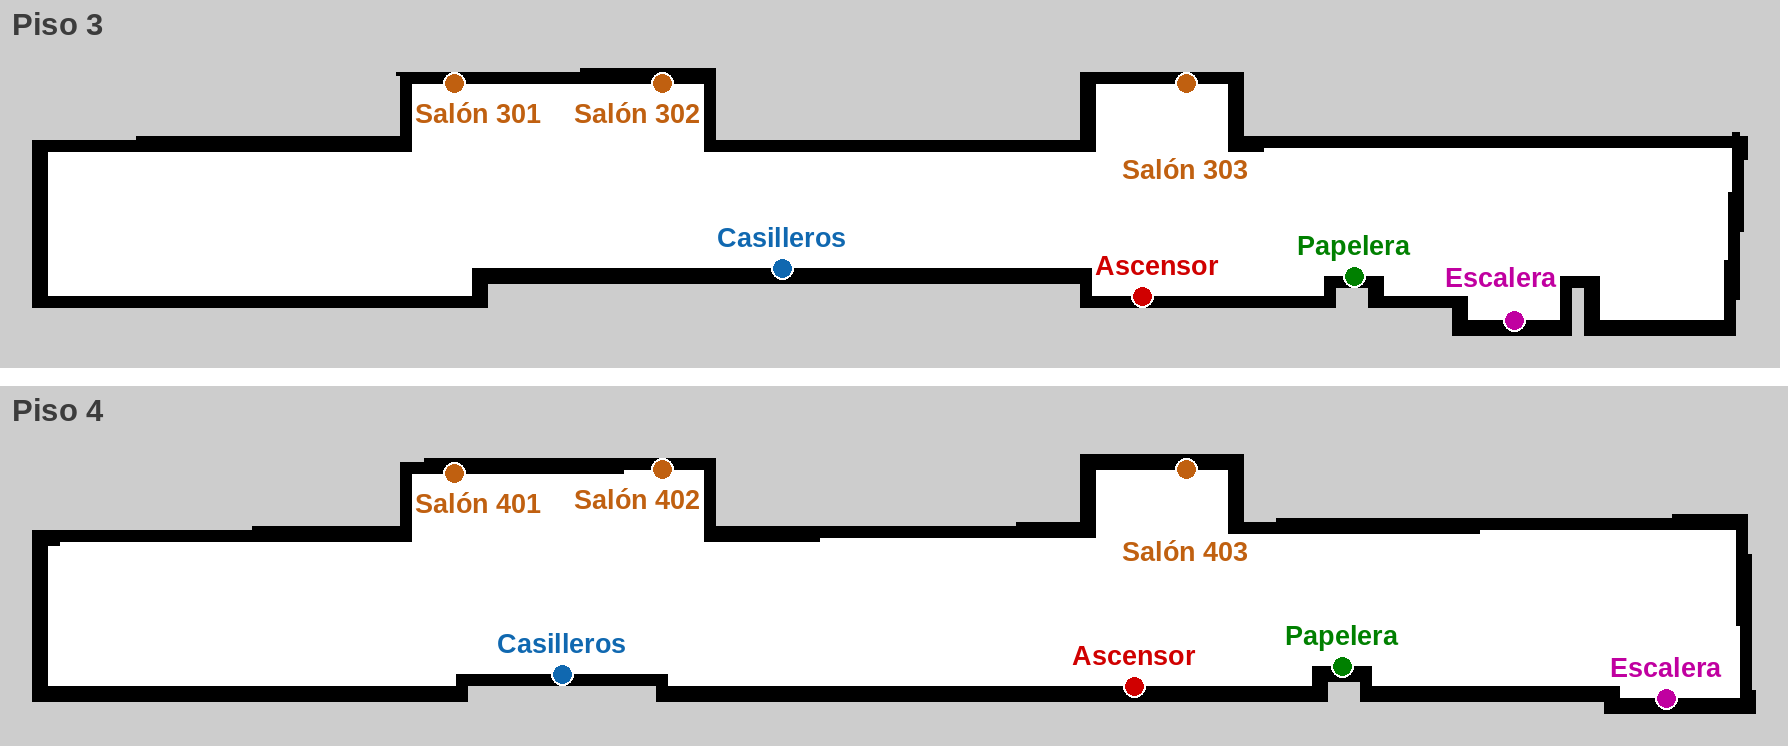
\includegraphics[width=0.86\textwidth]{imagenes/mapas_catalayud.png}
  \caption{Mapas de navegación de los pisos 3 (arriba) y 4 (abajo) del edificio Catalayud, derivados del levantamiento con flexómetro, con el extremo norte a la izquierda.}
  \label{fig:mapas-catalayud}
\end{figure}

\subsection{Arquitectura general y módulos}

La arquitectura consta de una interfaz web por la que entra la solicitud, un coordinador que la reparte y dos agentes, uno por piso, con su pila de navegación (figura~\ref{fig:arquitectura}). Ningún agente atraviesa la zona de transición: la cruza el usuario, y lo que se traspasa entre agentes en la escalera es la responsabilidad de guiarlo.

\begin{figure}[H]
  \centering
  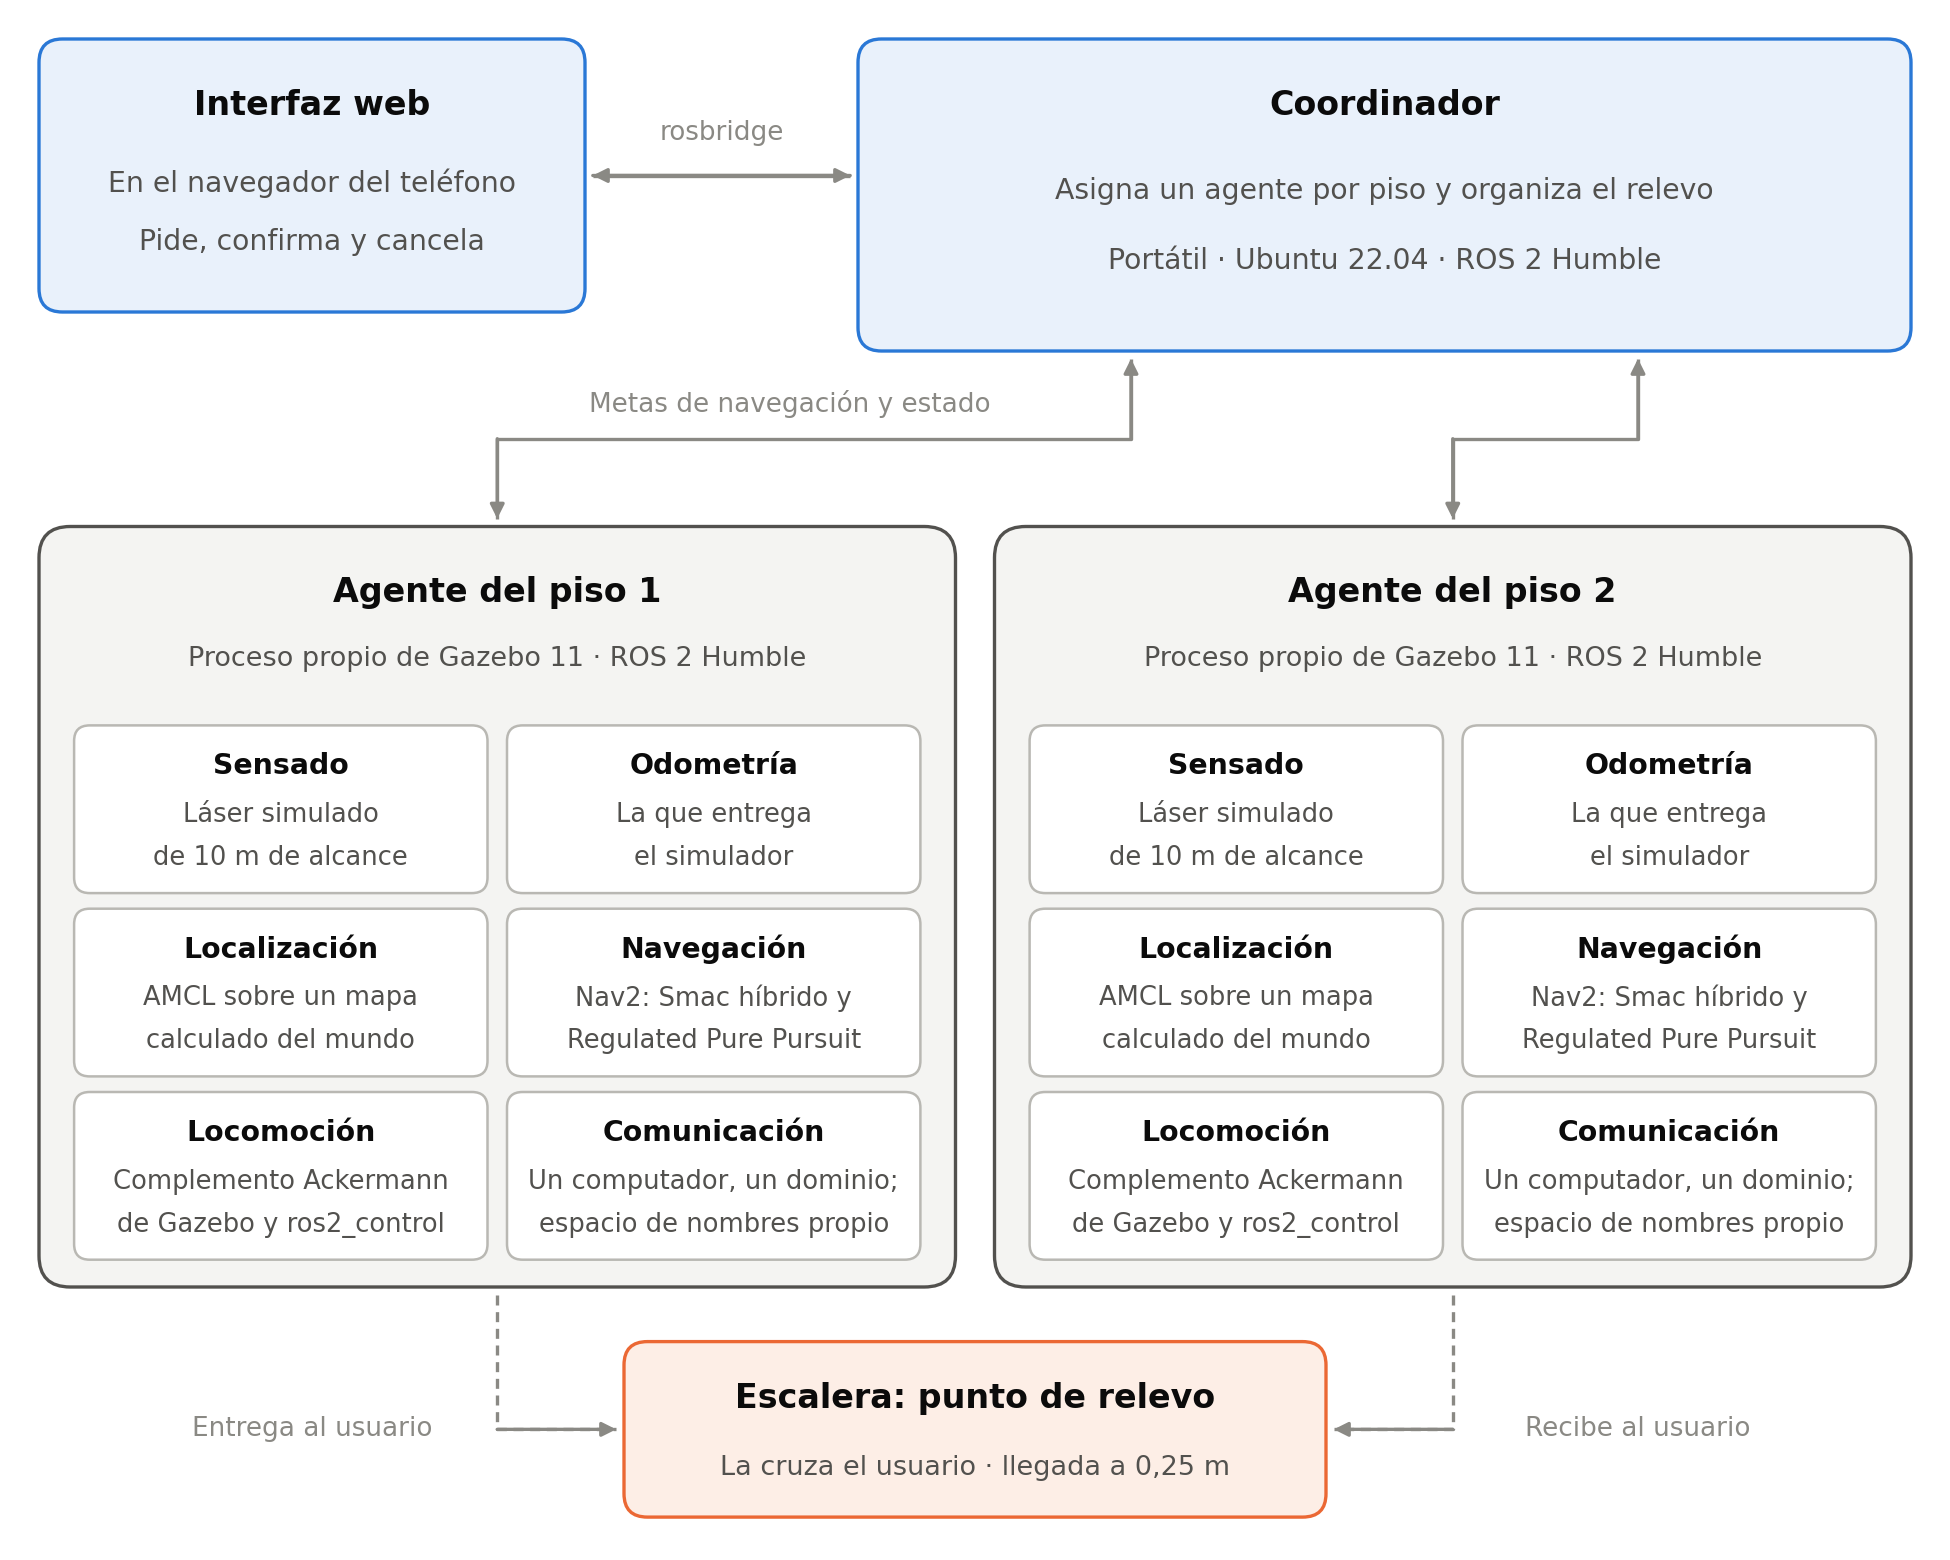
\includegraphics[width=0.78\textwidth]{imagenes/arquitectura_simulacion.png}
  \caption{Arquitectura del sistema en simulación.}
  \label{fig:arquitectura}
\end{figure}

Sus módulos son percepción, localización, planificación, control, locomoción, comunicación, coordinación e interfaz. Los cinco primeros se ejecutan en cada agente, la coordinación y la interfaz se sirven desde el portátil, y la comunicación los enlaza. La figura~\ref{fig:nodos} muestra los nodos principales en la campaña con los agentes físicos y lo que circula entre ellos. Los dos agentes son iguales, los componentes del fabricante van en borde discontinuo y las flechas siguen el sentido de los datos, con el nombre del tópico, servicio o acción. El navegador pide la ruta al planificador y su seguimiento al controlador, y la pose que estima \texttt{amcl} llega a los demás nodos por las transformadas. El anexo C enlaza el grafo completo, obtenido en simulación.

El funcionamiento se definió como un escenario de relevo en siete pasos. El usuario hace la solicitud, el coordinador asigna el agente y el agente del piso de origen recoge al usuario y lo guía hasta la escalera, donde lo entrega. El coordinador notifica entonces al agente del otro piso, que va a su punto de transferencia, el sistema espera a que el usuario confirme que cambió de piso y el guiado se reanuda en el piso de destino.

\begin{figure}[H]
  \centering
  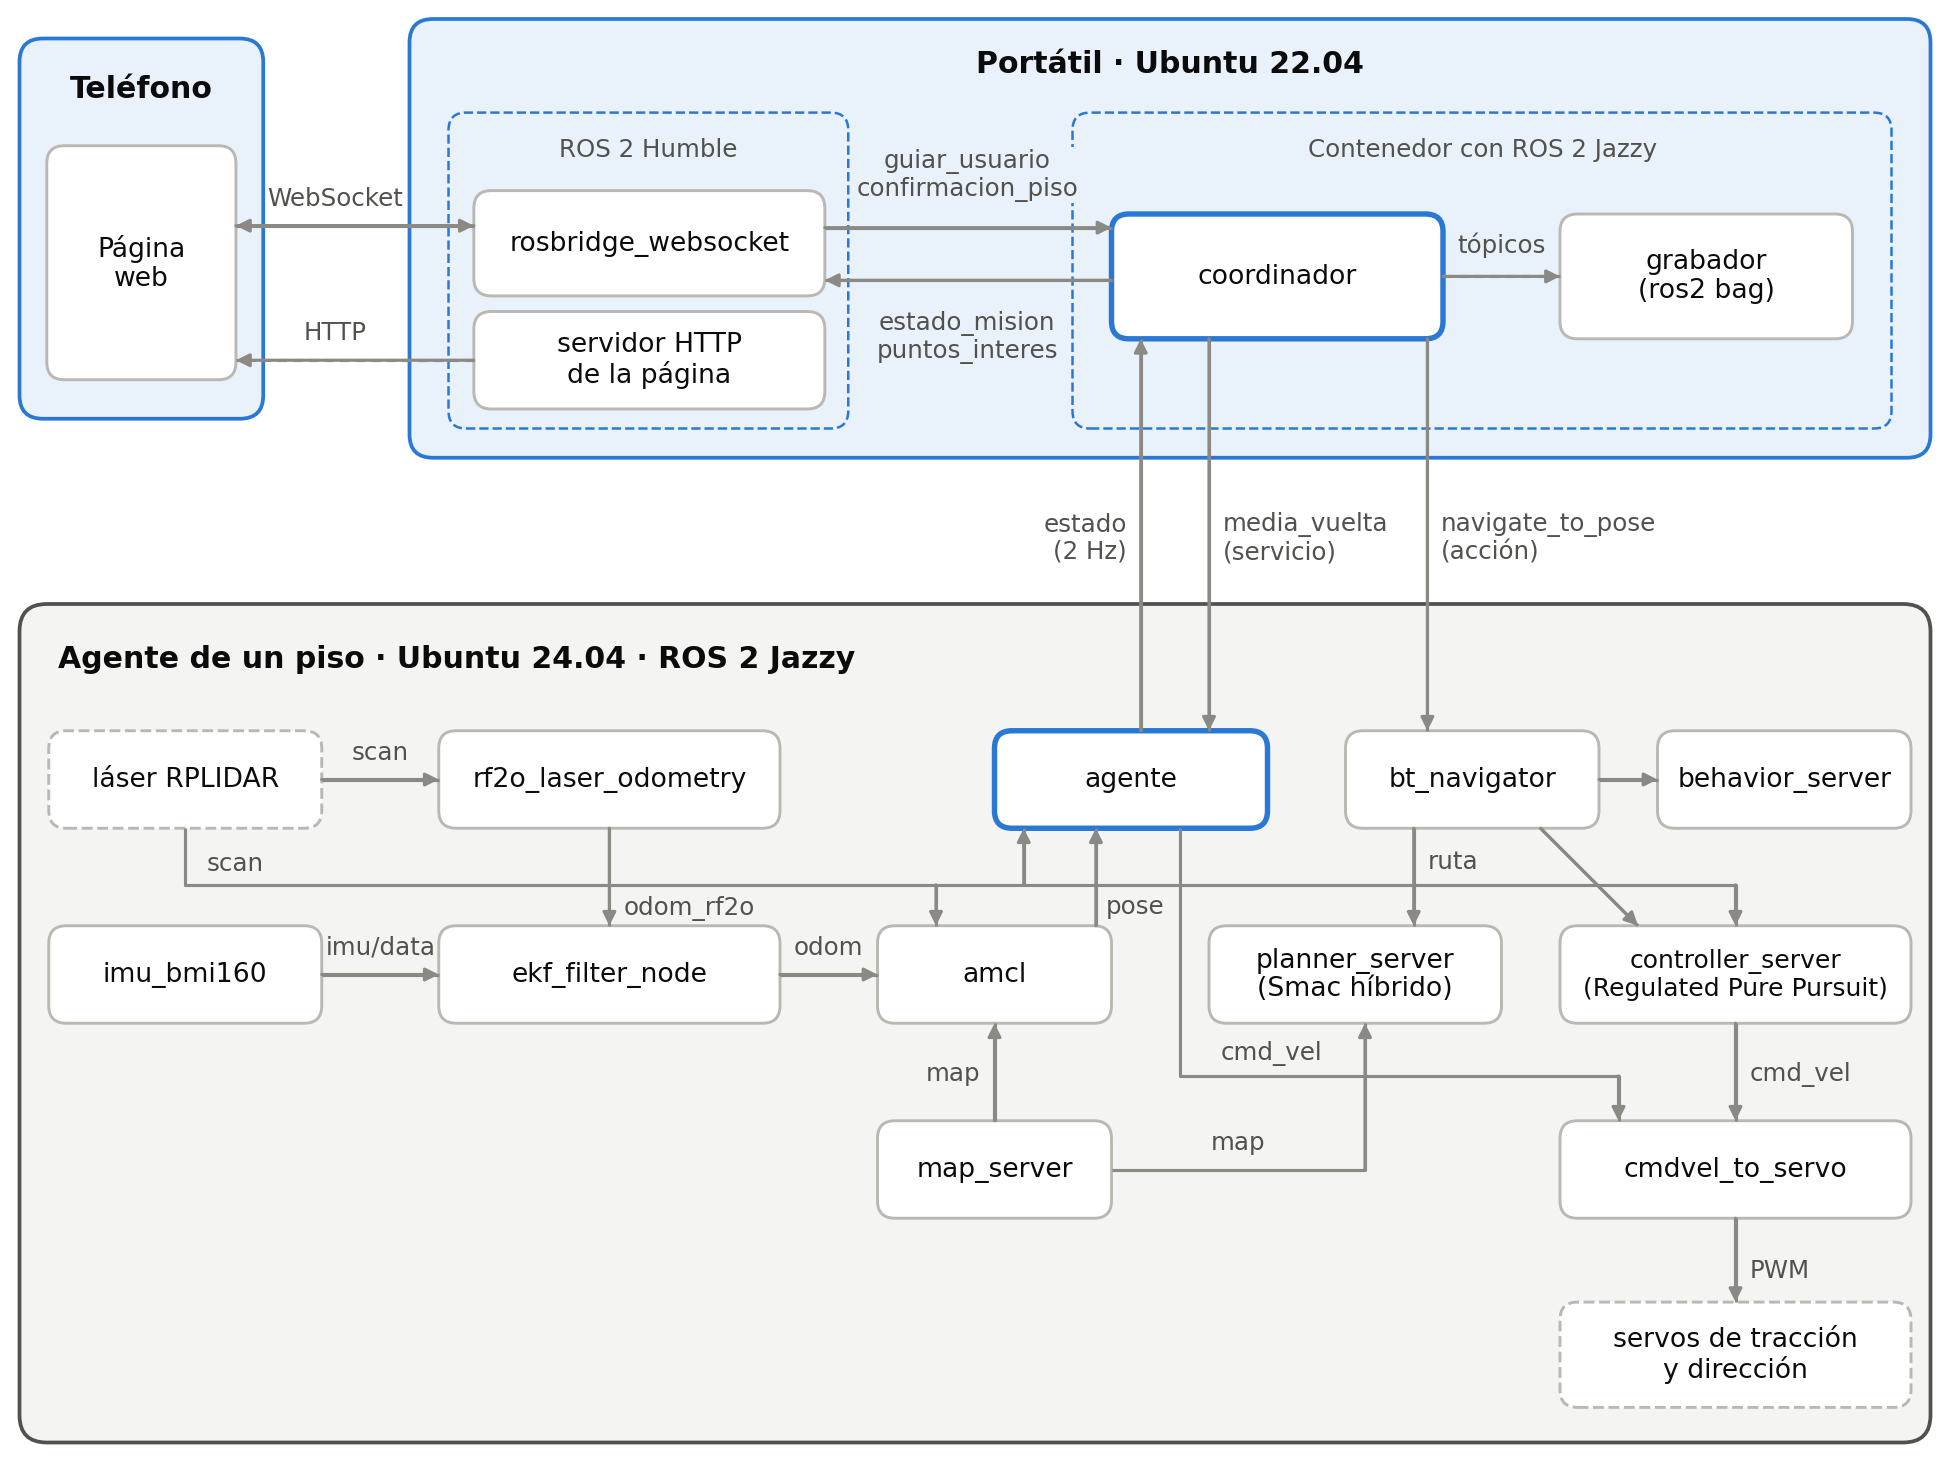
\includegraphics[width=0.82\textwidth]{imagenes/nodos_sistema.png}
  \caption{Nodos principales de ROS~2 en la campaña con los agentes físicos.}
  \label{fig:nodos}
\end{figure}

\subsection{Estrategia de asignación de tareas}
\label{sec:planificador}
\label{sec:asignacion}

Cada piso tiene un agente asignado, y esa correspondencia es un dato de configuración, sin estar fija en el código. El coordinador elige el agente al aceptar la solicitud, según el piso del origen y del destino (anexo A, video 5). En los agentes físicos, además, comprueba la llegada con la pose que publica el agente, sin darla por buena solo porque Nav2 la informe.

El relevo es el aporte declarado del proyecto, de modo que su planificación se escribió como una función pura, sin dependencia de ROS~2 ni estado propio (figura~\ref{fig:planificador}). Entran el catálogo de puntos y un par origen-destino, y salen los tramos que hay que ejecutar o un error con su motivo, antes de que ningún agente se mueva. Si el origen y el destino están en el mismo piso, la misión tiene dos tramos del mismo agente: ir a recoger al usuario y llevarlo al destino. Si están en pisos distintos, tiene cuatro: los dos anteriores, terminando en el punto de transferencia del piso de origen; el desplazamiento del segundo agente a su punto de transferencia; y el guiado final. El punto de encuentro no se negocia, puesto que es el punto de transferencia declarado de cada piso en el catálogo.

\begin{figure}[H]
  \centering
  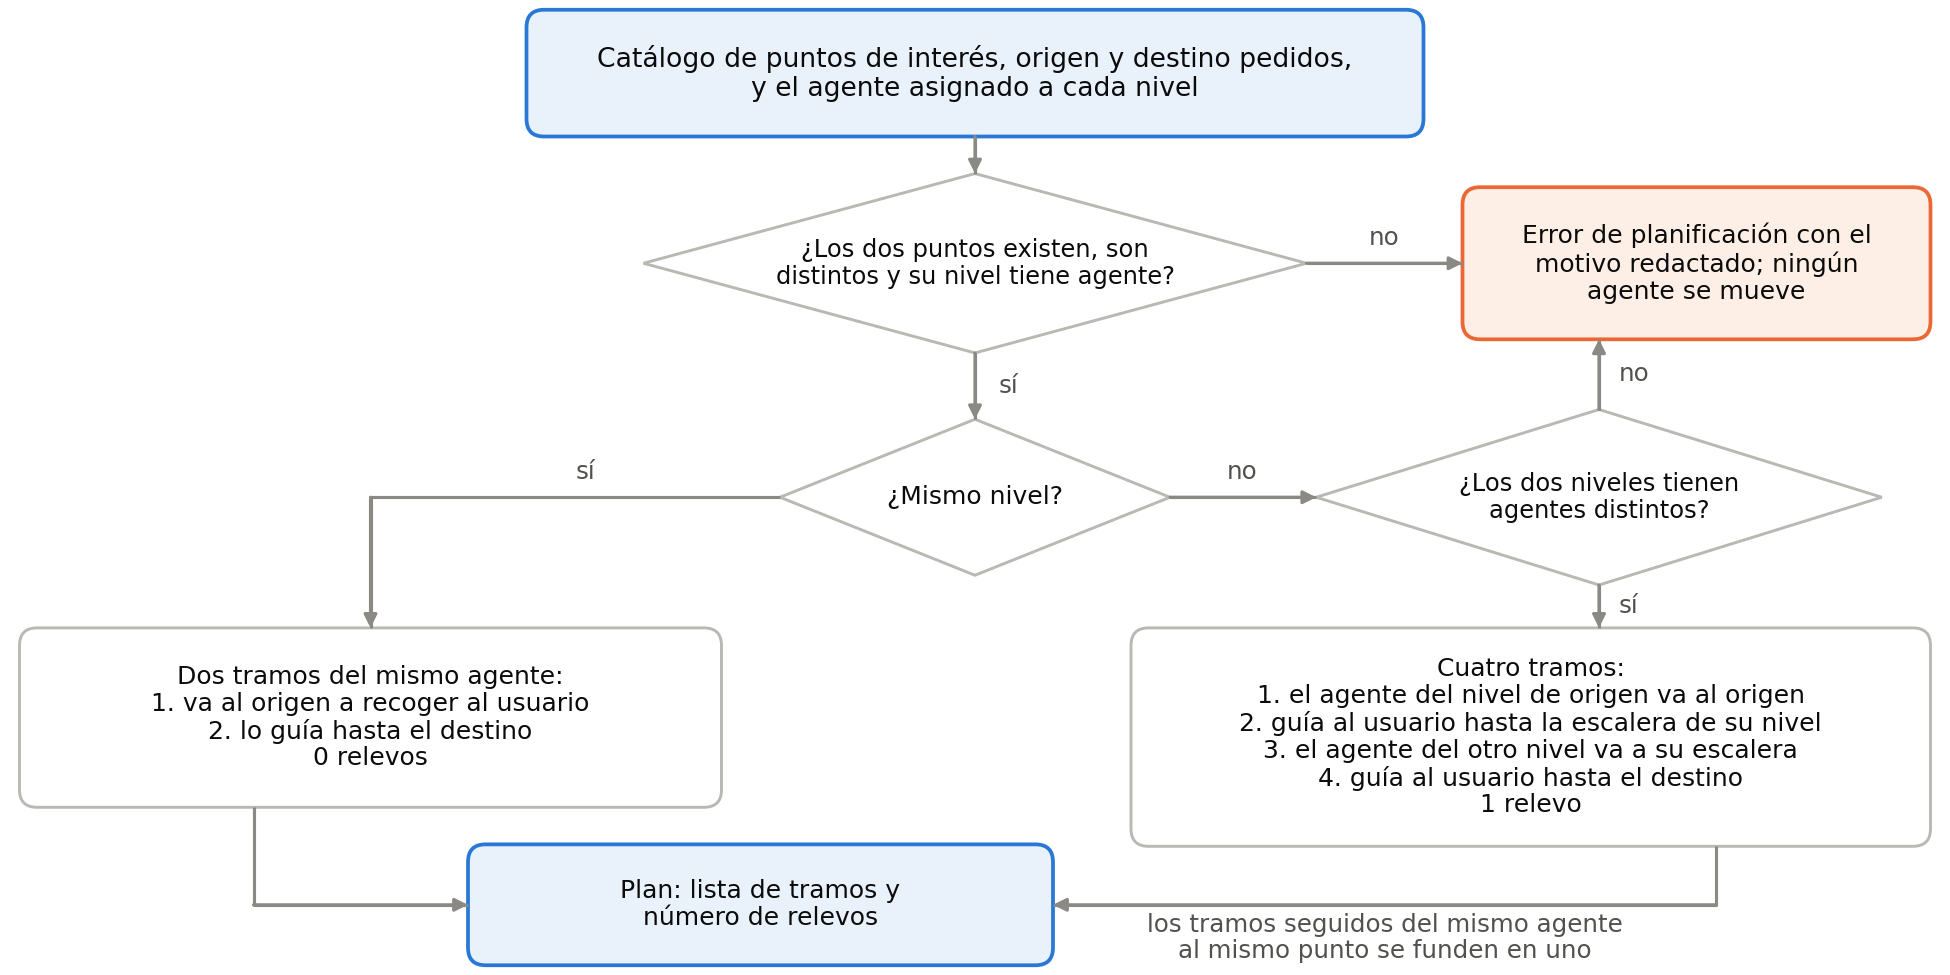
\includegraphics[width=0.68\textwidth]{imagenes/planificador.png}\hspace*{0.76cm}
  \caption{Función que planifica una misión.}
  \label{fig:planificador}
\end{figure}

Con el relevo dentro del nodo, mezclado con los clientes de acción, la única forma de comprobarlo habría sido levantar dos simuladores y observar si el agente llega. Como función pura, en cambio, una prueba automática la recorre entera en milisegundos y sin simulador. El catálogo de los pisos 2 y 3 del edificio Gregorio tiene 31 puntos de interés, quince en el piso 2 y dieciséis en el piso 3, y cada par ordenado de dos puntos distintos es una solicitud posible: $31 \times 30 = 930$ combinaciones. La prueba planifica las 930 y comprueba en todas que el plan empieza en el origen y termina en el destino, que ningún agente recibe una meta fuera de su piso, que una misión de un solo piso usa un agente y ningún relevo, y que una de dos pisos usa los dos agentes y un relevo. Con ella se encontró, y se corrigió, un defecto que una ejecución no habría mostrado: cuando el origen o el destino era el propio punto de transferencia de su piso, el plan mandaba al mismo agente dos veces a la misma pose. Como Nav2 devuelve éxito al instante ante un desplazamiento de cero metros, en simulación no se habría visto.

El planificador exige además un único punto de transferencia por piso y falla con un mensaje explícito si encuentra dos. Como cada piso tiene una escalera, la condición se cumple, y la verificación obliga a tomar la decisión a la vista si algún día hubiera dos.

\subsection{Esquema de comunicación entre agentes}
\label{sec:contrato}

El esquema se fijó, antes de escribir código, en un contrato que define qué habla con qué y en qué formato (tabla~\ref{tab:contrato}), implementado como un paquete propio de mensajes de ROS~2. Un coordinador decide y manda, dos agentes, uno por piso, ejecutan, y una interfaz web es la vía por la que el usuario pide el servicio. La comunicación sigue tres reglas:

\begin{enumerate}[leftmargin=*]
  \item El coordinador manda a un agente solo mediante la acción de navegación de ROS~2 o la petición de una media vuelta, que el agente ejecuta por su cuenta antes de navegar; no publica velocidades directamente.
  \item La interfaz habla solo con el coordinador, nunca con los agentes.
  \item El texto que ve el usuario lo redacta el coordinador, y la interfaz lo muestra literal.
\end{enumerate}

La tercera regla evita duplicar la lógica: si la página interpretara el estado para decidir qué mostrar, habría dos copias de la misma lógica, que con el tiempo acabarían contradiciéndose. La acción de guiado recibe el origen y el destino, devuelve el estado durante la misión y, al final, el tiempo total y el número de relevos o el motivo del fallo. Cada cambio de etapa (tabla~\ref{tab:etapas-mision}) se publica, y esas publicaciones son las marcas de tiempo con que se calculan las métricas.

\begin{table}[H]
  \centering\footnotesize\setstretch{1.0}
  \caption{Interfaces del contrato entre la interfaz web, el coordinador y los agentes, donde \texttt{N} es el número del agente: 1 en el piso inferior y 2 en el superior.}
  \label{tab:contrato}
  \begin{tabular}{@{}>{\scriptsize\raggedright\arraybackslash}p{0.285\textwidth}>{\raggedright\arraybackslash}p{0.12\textwidth}>{\raggedright\arraybackslash}p{0.195\textwidth}>{\raggedright\arraybackslash}p{0.32\textwidth}@{}}
    \toprule
    \footnotesize\textbf{Interfaz} & \textbf{Tipo} & \textbf{Sentido} & \textbf{Contenido} \\ \midrule
    \texttt{/coordinacion/guiar\_usuario} & acción propia & interfaz $\rightarrow$ coordinador & Origen y destino; estado durante la misión; éxito, tiempo, relevos o motivo del fallo \\
    \texttt{/coordinacion/estado\_mision} & tópico propio, 1~Hz & coordinador $\rightarrow$ interfaz & Etapa, agente activo, destino, distancia restante y texto para el usuario \\
    \texttt{/coordinacion/puntos\_interes} & tópico persistente & coordinador $\rightarrow$ interfaz & Catálogo de puntos de interés, con su piso \\
    \texttt{/coordinacion/confirmacion\_piso} & tópico de texto & interfaz $\rightarrow$ coordinador & Confirmación del cambio de piso \\
    \texttt{/robotN/navigate\_to\_pose} & acción de Nav2 & coordinador $\rightarrow$ agente & Meta de cada tramo \\
    \texttt{/robotN/media\_vuelta} & servicio & coordinador $\rightarrow$ agente & Media vuelta antes de una meta que queda detrás \\
    \texttt{/robotN/estado} & tópico propio, 2~Hz & agente $\rightarrow$ coordinador & Piso, pose en el mapa y estado del agente \\
    \texttt{/robotN/odom} & odometría & agente $\rightarrow$ coordinador & Desplazamiento, para marcar el primer movimiento \\ \bottomrule
  \end{tabular}
\end{table}

\begin{table}[H]
  \centering\footnotesize\setstretch{1.0}
  \caption{Etapas de una misión, tal como las publica el coordinador.}
  \label{tab:etapas-mision}
  \begin{tabular}{@{}>{\raggedright\arraybackslash}p{0.27\textwidth}>{\raggedright\arraybackslash}p{0.65\textwidth}@{}}
    \toprule
    \textbf{Etapa} & \textbf{Significado} \\ \midrule
    Recibida & El coordinador aceptó la solicitud y todavía no asignó agente \\
    Primer tramo & El agente del piso de origen va a recoger al usuario y lo guía \\
    Transferencia & El agente del otro piso va a su punto de transferencia \\
    Esperando confirmación & El sistema espera que el usuario confirme que ya cambió de piso \\
    Segundo tramo & El agente del piso de destino guía al usuario hasta el final \\
    Completada & La misión terminó con la llegada verificada \\
    Fallida & La misión terminó sin cumplirse, con el motivo en el texto \\
    Cancelando & El usuario canceló y el agente activo regresa a su punto de transferencia \\
    Inactiva & No hay misión en curso \\ \bottomrule
  \end{tabular}
\end{table}

% =====================================================================
\section{Segundo objetivo específico: plataforma robótica}
\label{sec:plataforma}

La plataforma se construyó sobre dos agentes AWS DeepRacer (figura~\ref{fig:agentes-fisicos}), cada uno a cargo de un piso del edificio Catalayud, integrando los módulos de locomoción, sensado, procesamiento y comunicación que nombra el objetivo. La tabla~\ref{tab:vehiculo} reúne los componentes del sistema, incluidos los de la red. El láser que traía el kit no era el que describía el primer informe de hardware, y se identificó leyendo el modelo que informa el propio sensor.

\begin{table}[H]
  \centering\footnotesize\setstretch{1.0}
  \caption{Lista de componentes del sistema.}
  \label{tab:vehiculo}
  \begin{tabular}{@{}>{\raggedright\arraybackslash}p{0.23\textwidth}c>{\raggedright\arraybackslash}p{0.62\textwidth}@{}}
    \toprule
    \textbf{Componente} & \textbf{Cant.} & \textbf{Descripción} \\ \midrule
    \multicolumn{3}{@{}l}{\textit{Agentes}} \\
    Chasis & 2 & AWS DeepRacer, escala 1:18, dirección Ackermann, motor de tracción con variador y servomotor de dirección \\
    Tarjeta de cómputo & 2 & Tarjeta original, procesador Intel Atom E3930 de dos núcleos, 4~GB de memoria; Ubuntu 24.04 y ROS~2 Jazzy \\
    Láser & 2 & RPLIDAR A1M8-R5, por USB: 360$^\circ$, 360 muestras por barrido, alcance de 0,15 a 12~m, entre 6,8 y 7~Hz \\
    Unidad inercial & 2 & Bosch BMI160 integrada en la tarjeta, por I2C: giroscopio y acelerómetro \\
    Cámaras & 2 pares & Estéreo; desactivadas por software: el sistema no las usa y cargaban la tarjeta \\
    Batería de cómputo & 2 & Alimenta la tarjeta \\
    Batería de tracción & 2 & Polímero de litio \\ \addlinespace
    \multicolumn{3}{@{}l}{\textit{Coordinación e interacción}} \\
    Portátil & 1 & Ubuntu 22.04 y ROS~2 Humble (AMD Ryzen 5 PRO 5650U, 16~GB); el coordinador se ejecuta en un contenedor con Jazzy \\
    Teléfono & 1 & Abre la interfaz web, conectado a la red de los agentes \\ \addlinespace
    \multicolumn{3}{@{}l}{\textit{Red}} \\
    Enrutador & 1 & TP-Link TL-WR940N: reparte las direcciones de la red y da un enlace de respaldo a 2,4~GHz \\
    Puntos de acceso & 2 & FiberHome, uno por piso del edificio Catalayud, en modo puente: 5~GHz, canal 44 en el piso 3 y 36 en el piso 4 \\
    Cables de red & 2 & Del enrutador a cada punto de acceso, entre puertos LAN: uno en el mismo piso y otro entre pisos \\ \addlinespace
    \multicolumn{3}{@{}l}{\textit{Medición}} \\
    Flexómetro & 1 & Levantamiento de las plantas y medida del avance y de la llegada en las pruebas de odometría y de navegación \\ \bottomrule
  \end{tabular}
\end{table}

\begin{figure}[H]
  \centering
  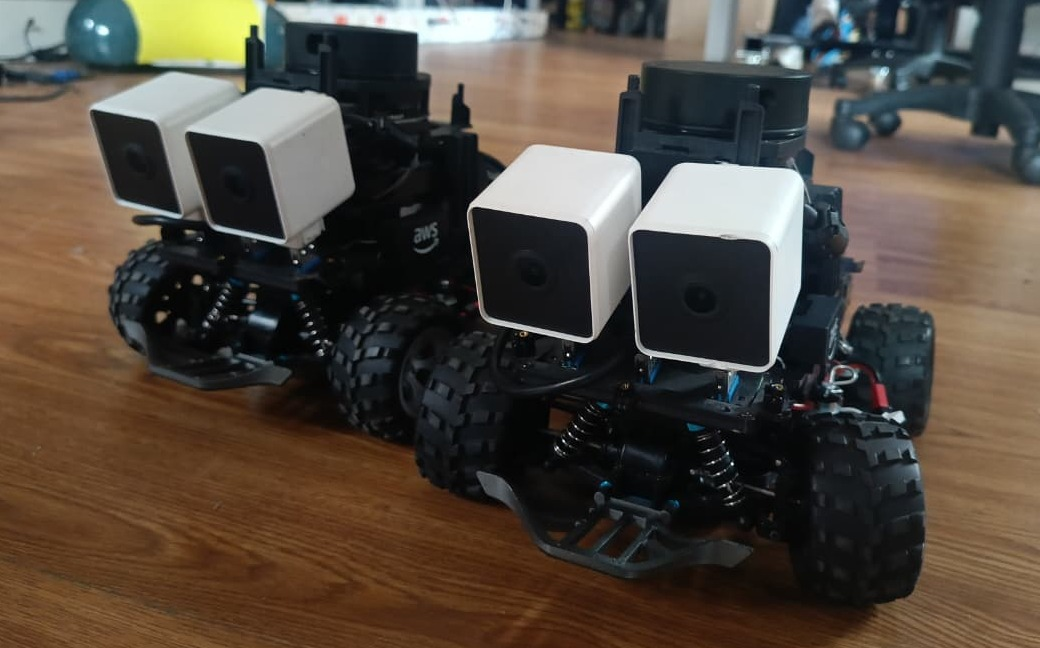
\includegraphics[width=0.52\textwidth]{imagenes/agentes_fisicos.jpg}
  \caption{Los dos agentes físicos, construidos sobre la plataforma AWS DeepRacer.}
  \label{fig:agentes-fisicos}
\end{figure}

\subsection{Selección de la plataforma y del simulador}
\label{sec:donkeycar}

El anteproyecto planteó construir los agentes sobre DonkeyCar, una plataforma abierta de vehículos a escala con dirección tipo automóvil, orientada a la conducción autónoma con una cámara \autocite{donkeycar}, con una Raspberry Pi~4, simulación en CoppeliaSim y visión con OpenCV. Para analizarla se instaló su simulador, que se condujo desde la interfaz web de la plataforma, y se empezó un modelo propio del agente para ROS~2, con el chasis, las ruedas, la dirección y su árbol de transformaciones (figura~\ref{fig:donkeycar}).

Con ese trabajo se identificaron las limitaciones de la plataforma. Su ecosistema no se actualiza desde hace años y no es compatible con las versiones recientes de ROS~2. Su simulador tampoco se comunica con ROS~2, de modo que no permite probar el mapeo, la localización, la planificación ni la comunicación entre agentes, que son el núcleo del proyecto. Además, no existía un modelo para Gazebo con dirección Ackermann que funcionara en ROS~2 Humble.

\begin{figure}[H]
  \centering
  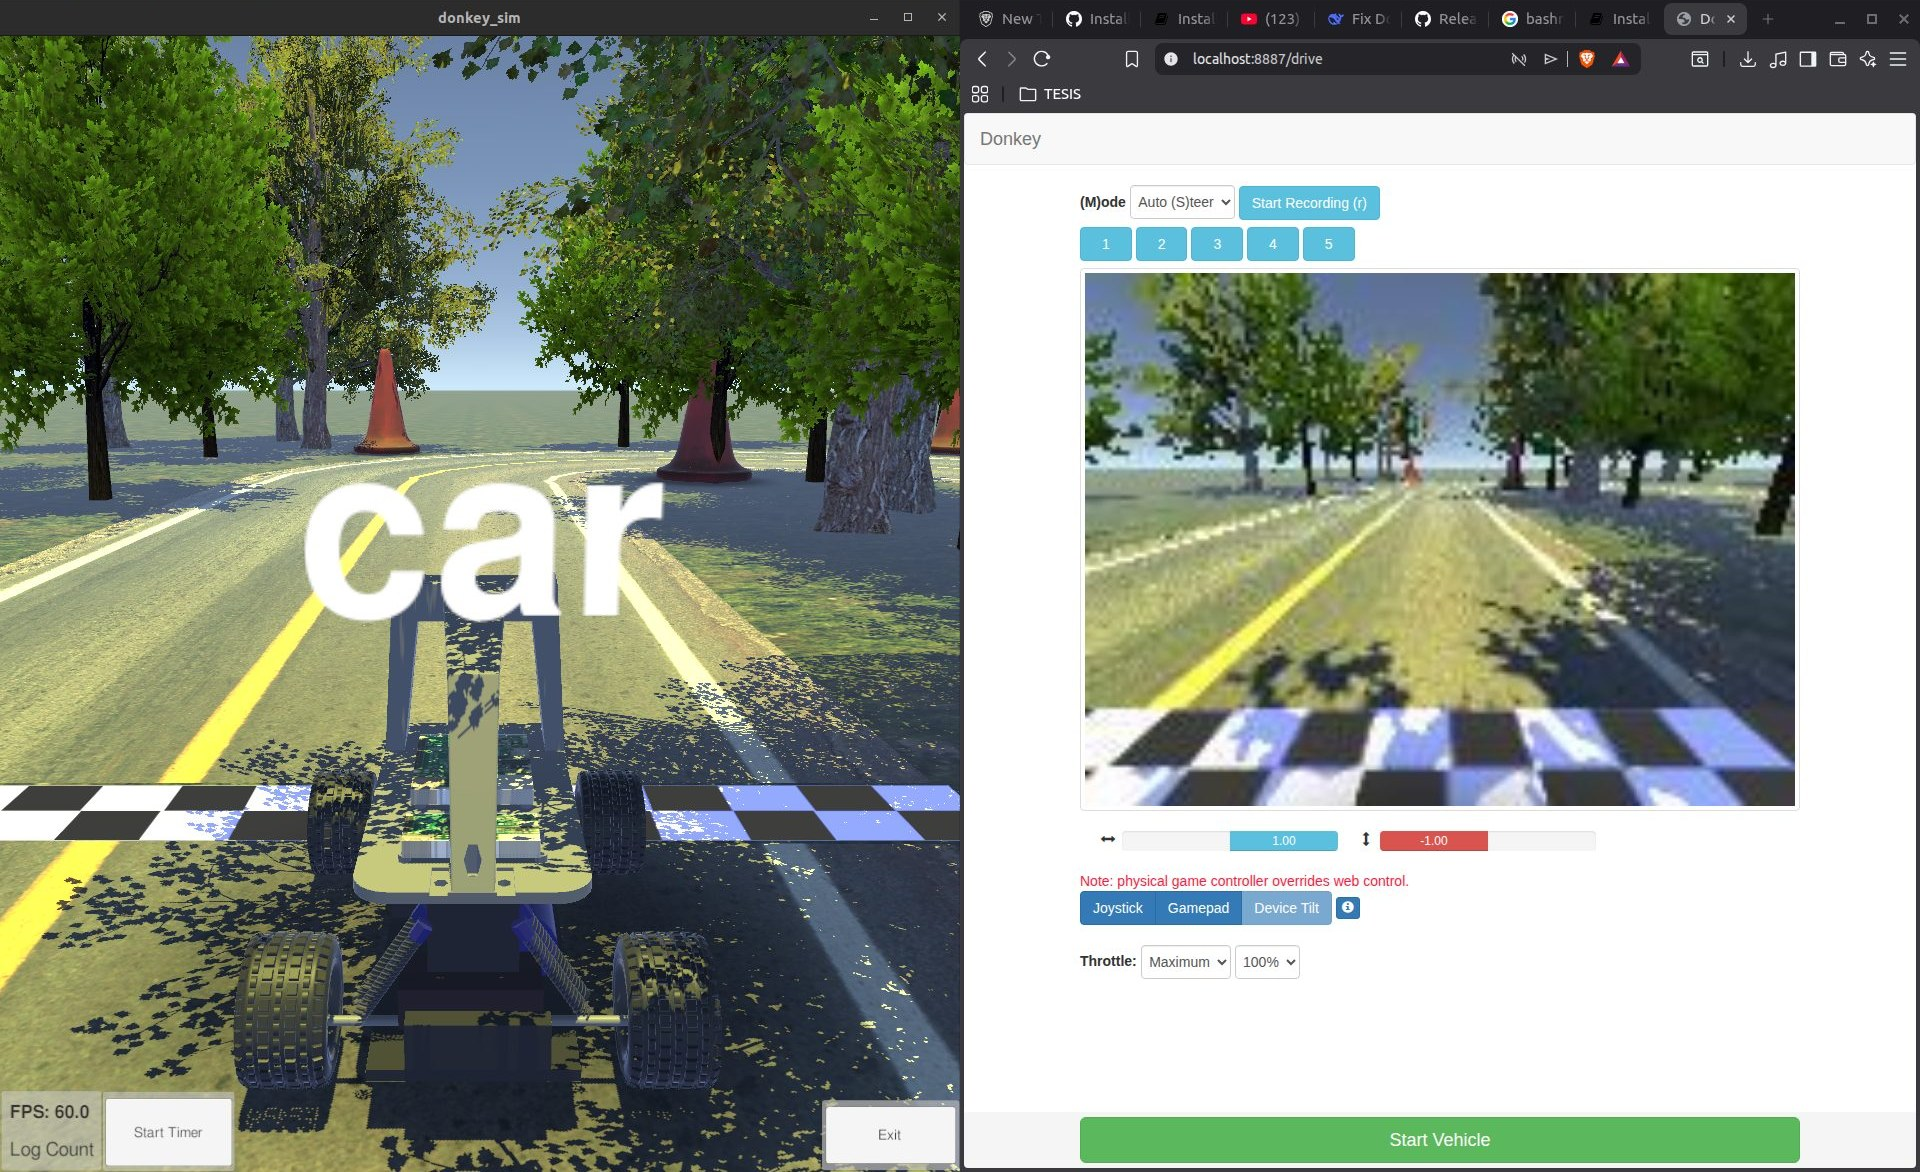
\includegraphics[height=4.6cm]{imagenes/etapa_donkeycar_simulador.jpg}\hfill
  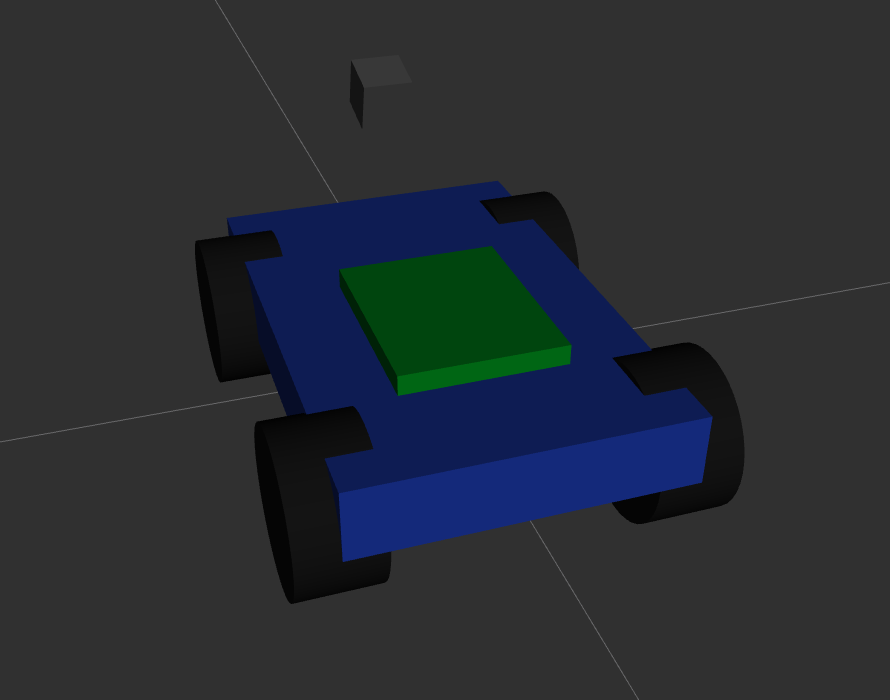
\includegraphics[height=4.6cm]{imagenes/etapa_donkeycar_modelo.png}
  \caption{Exploración de la plataforma DonkeyCar: su simulador (izquierda) y el modelo propio del agente en el visualizador de ROS~2 (derecha).}
  \label{fig:donkeycar}
\end{figure}

Para el simulador se fijaron cuatro criterios: compatibilidad con ROS~2 Humble, vehículos con dirección Ackermann, entornos interiores y soporte para mapeo y navegación. Entre CoppeliaSim, que proponía el anteproyecto, el simulador del curso F1TENTH y Gazebo \autocite{koenig2004gazebo}, se eligió Gazebo por su integración directa con ROS~2 y con su sistema de control de articulaciones.

Como plataforma se adoptó AWS DeepRacer, la decisión que hizo viable el proyecto en el tiempo disponible. Es la misma clase de vehículo que el DonkeyCar, con chasis a escala 1:18, dirección Ackermann, computador a bordo y software abierto, y AWS publicó en código abierto su modelo de simulación, con un complemento de cinemática Ackermann para Gazebo y los nodos que traducen las órdenes de velocidad a los servos \autocite{awsdeepracer2021}. Además, la universidad ya tenía dos. Lo que pide el segundo objetivo, que es cinemática tipo automóvil, bajo costo y código modificable, se cumple igual con las dos plataformas, y usar las que existían dejó el tiempo para la coordinación. El costo fue convivir con el software del fabricante, cuyos nodos ocupan el láser, se ejecutan con el usuario administrador y publican sin espacio de nombres.

El software de la comunidad de AWS DeepRacer \autocite{deepracercustomcar} se instaló en una Raspberry Pi~4 y en la tarjeta original, y los agentes quedaron con la tarjeta original, para la que ese software solo se publica sobre Ubuntu 24.04 y ROS~2 Jazzy. Como la integración de Gazebo~11 con ROS~2 no está publicada para Jazzy, el proyecto trabaja con dos distribuciones.

\subsection{Locomoción}
\label{sec:banda-muerta}
\label{sec:media-vuelta}

En simulación, el software de AWS, escrito para ROS~2 Foxy sobre Ubuntu 20.04, se migró a Humble sobre Ubuntu 22.04 con tres cambios en el sistema de control de articulaciones: la orden que activa los controladores pasó de \texttt{start} a \texttt{active}, y el componente que publica el estado de las articulaciones cambió de nombre y de tipo. En un mundo vacío (figura~\ref{fig:deepracer-sim}, izquierda), el modelo funcionó con el láser y la cámara publicando a 62 cuadros por segundo, un factor de tiempo real de 1,00 y los siete controladores activos, y la odometría registró 0,40~m/s ante una orden de 0,5~m/s. También se corrigió el modelo del agente, que tomaba la velocidad angular de la orden estándar de ROS~2 como el ángulo del volante. El ángulo se calcula ahora con el modelo de bicicleta, a partir de las velocidades angular y lineal y de la distancia entre ejes, con lo que el error de seguimiento de las trayectorias bajó a la mitad, y la misma corrección se aplicó al nodo que mueve al agente físico.

\begin{figure}[H]
  \centering
  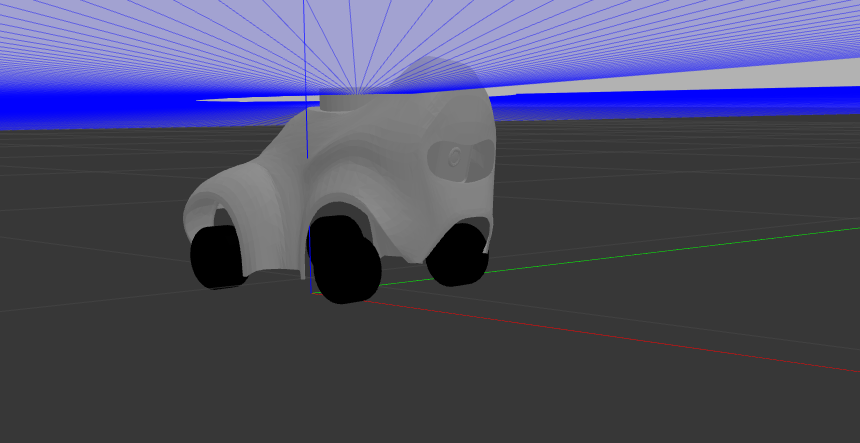
\includegraphics[height=4.4cm]{imagenes/etapa_deepracer_gazebo.png}\hfill
  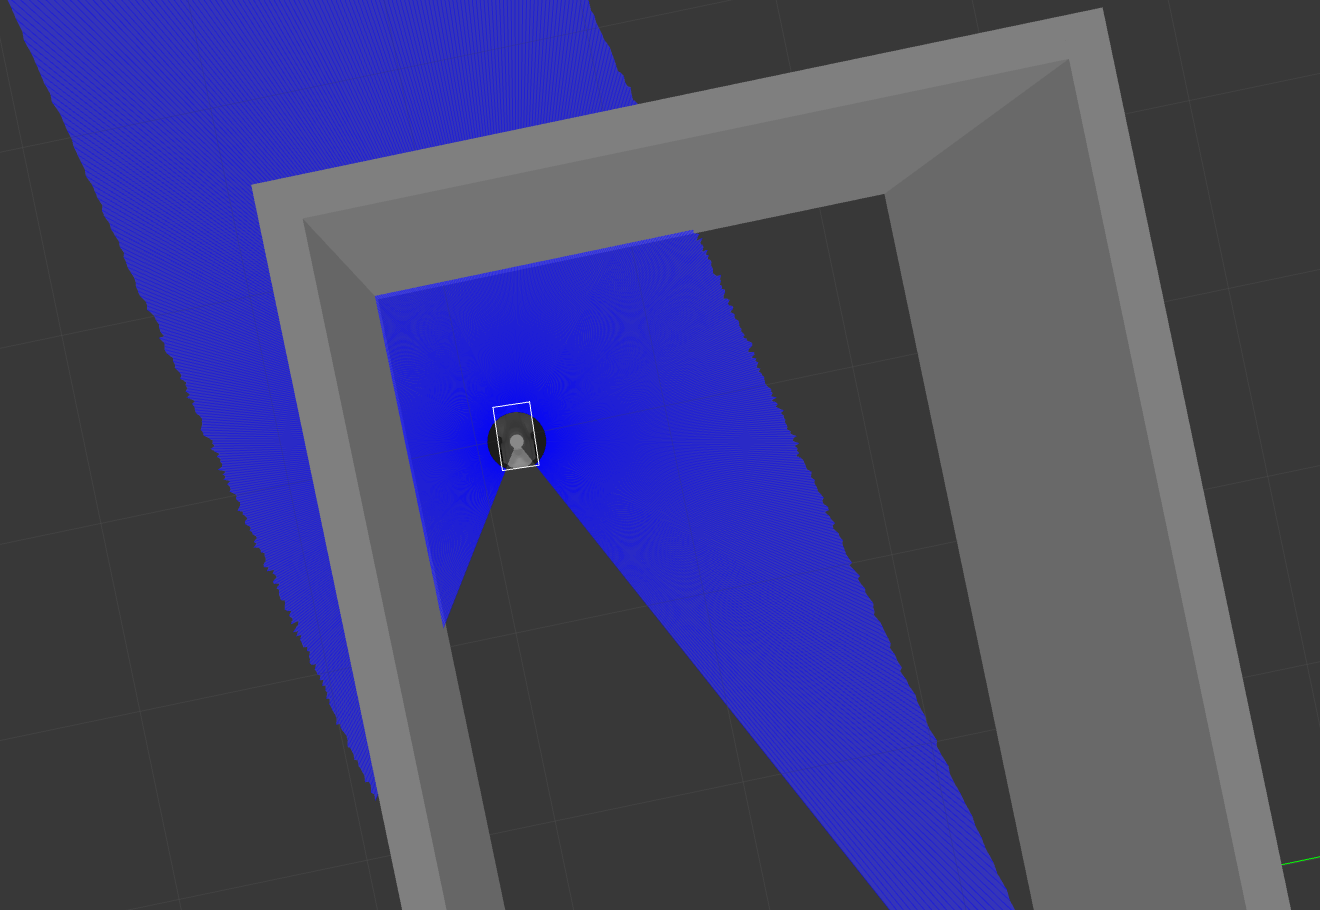
\includegraphics[height=4.4cm]{imagenes/etapa_pasillo_usta.png}
  \caption{Modelo de AWS DeepRacer en ROS~2 Humble: en un mundo vacío (izquierda) y en el primer modelo del pasillo de la universidad (derecha).}
  \label{fig:deepracer-sim}
\end{figure}

En los agentes físicos, cuya marcha se comprobó primero desde su interfaz web (anexo A, video 3), un puente traduce la orden de velocidad al variador y al servomotor. Al integrar esa cadena apareció una característica de la plataforma que condiciona la llegada, la banda muerta de tracción: el agente no se mueve con velocidades pedidas por debajo de 0,40~m/s. El puente convertía esas órdenes en tracción nula, sin ningún aviso, y el agente se detenía al entrar en la fase final del recorrido. Se subió a 0,40~m/s la velocidad mínima de aproximación del controlador, y después se modificó el puente para que envíe las órdenes menores con el escalón de tracción más bajo. Como resultado, el agente se aproxima a la meta a 0,40~m/s y no tiene régimen de aproximación fina, un límite de la plataforma que no se corrige afinando el controlador.

Además, como la tracción funciona en lazo abierto, la relación entre la orden y la velocidad real no es igual en los dos agentes, por lo que el puente tiene una escala por agente, ajustada en campo: 0,85 en el del piso 3 del edificio Catalayud y 0,9 en el del piso 4. Con la escala 1,0, el del piso 4 iba a 1,36~m/s y se pasaba de la meta; con 0,9 va a 0,74~m/s. Con la misma orden el motor retrocedía a 1,7 veces la velocidad de avance, de manera que la marcha atrás lleva una escala de 0,75.

La media vuelta es necesaria, puesto que cada misión empieza donde terminó la anterior y el siguiente usuario queda a menudo detrás del agente, que en pasillos de 2,5 a 3,2~m de ancho tiene que dar la vuelta en varios tiempos. En simulación la resuelve Nav2 con una inversión de marcha (anexo A, video 4), pero en el piso 4 de Catalayud, a la salida del pasillo de 2,5~m, abortó dos veces contra la pared, debido a que el planificador proponía cada segundo una maniobra distinta. Por esa razón se escribió una maniobra propia del agente, en lugar de seguir ajustando Nav2, que en ese caso trabajaba en el límite de lo que su controlador resuelve. La maniobra alterna marcha atrás y avance con la dirección a tope y empieza hacia el costado con más espacio. Cada tiempo se corta cuando la huella prevista del agente queda a menos de 0,10~m de un obstáculo, visto por el láser o marcado en el mapa, donde la escalera está cerrada, ya que el láser no ve su borde. El coordinador la pide antes de una meta que queda a más de 110$^\circ$ del rumbo del agente y a más de 1,5~m, y si no se completa en 120~s, sigue Nav2. En sus primeras pruebas giró 160$^\circ$ y 167$^\circ$, en un solo tiempo cada vez, y en la campaña con los agentes físicos se ejecutó 24 veces.

\subsection{Sensado}
\label{sec:odometria-laser}
\label{sec:imu}

El agente percibe con el láser, y como no tiene codificadores en las ruedas, su única odometría sale de comparar barridos sucesivos. En los pasillos rectos y uniformes del edificio Gregorio, donde cada barrido es casi igual al anterior, registró desde el 1,3~\% del avance real, en simulación, hasta el 73~\%, con un agente físico en el hall del piso 3, por falta de información en la señal. En los pisos 3 y 4 del edificio Catalayud, con la misma odometría y sin cambiar un parámetro, el error cayó por debajo del 5~\% (tabla~\ref{tab:odometria}), lo que hizo posible la demostración física.

El rumbo requirió la unidad inercial. Al principio también salía de la odometría del láser, que en un pasillo recto pierde los giros igual que el avance: con el agente quieto derivó hasta 5,9$^\circ$ por minuto, y un giro de 90$^\circ$ hecho a mano se registró como 19,1$^\circ$. La Bosch BMI160 de la tarjeta, que el software del fabricante no usa, midió giros de 90$^\circ$ y 360$^\circ$ con un error de 0,1~\% a 1,3~\%, y quieta no se desvió más de 0,3$^\circ$ en 60~s.

Se escribió un nodo que la lee y calibra el sesgo del giroscopio al arrancar, y un filtro de Kalman extendido toma de la odometría del láser el avance y de la unidad inercial el giro; la unidad publica a 25~Hz y el filtro se ejecuta a 15~Hz, para no cargar la tarjeta. En un giro de 90$^\circ$ contra una línea del piso, el filtro midió 90,17$^\circ$ en un agente y 88,38$^\circ$ en el otro, y con el agente quieto su rumbo se movió 0,3$^\circ$ o menos por minuto. La posición, en cambio, no mejora, ya que sigue saliendo del láser.

\subsection{Procesamiento y navegación autónoma}
\label{sec:primeros-entornos}
\label{sec:nav2-ackermann}

La navegación con mapa se adoptó después de evaluar un comportamiento reactivo. En un tramo simulado del pasillo de la universidad, de 7 por 3~m (figura~\ref{fig:deepracer-sim}, derecha; anexo A, video 1), donde el láser simulado no cubría el sector detrás del agente, se programó un seguidor de paredes como ejercicio de integración entre el láser y la cinemática del agente. La primera versión aplicaba control proporcional-derivativo sobre un rayo lateral del láser, pero saturaba el giro al no conocer la orientación del agente respecto a la pared, y la segunda usó la técnica de dos rayos del curso F1TENTH, que estima ese ángulo y la distancia a la pared un metro más adelante. Ninguna sintonía estabilizó al agente en ese tramo: el giro se saturaba y el agente trazaba círculos o chocaba, ya que su radio de giro deja muy poco margen en 3~m de ancho. En un pasillo ampliado de 15 por 5~m convergió por tramos, a 0,76~m de la pared frente a un objetivo de 0,5~m, y se perdía en los extremos. De estos ensayos se concluyó que un comportamiento reactivo no anticipa las restricciones de un vehículo tipo automóvil en un pasillo estrecho, por lo que el proyecto pasó a navegar con un mapa y con un planificador que conoce esas restricciones.

El primer entorno de esa navegación fue el modelo del piso 2 del edificio Gregorio, donde están los salones ETM: un pasillo de 44,25~m de largo y 5,09~m de ancho, en el que se comprobaron el láser, la cámara, la odometría y el árbol de transformaciones. Con ese mundo se construyó el primer mapa por localización y mapeo simultáneos (SLAM), que se aceptó sin medirlo y que, al medirlo después, resultó de 23,04 por 15,72~m, la mitad del largo y el triple del ancho del pasillo. Fue la primera manifestación, sin diagnóstico entonces, de la falta de información de avance en un pasillo recto, que acabó determinando cómo se hicieron los mapas.

Cada agente ejecuta su navegación a bordo, sobre Nav2, cuya configuración por omisión supone tracción diferencial y propone trayectorias que un vehículo tipo automóvil no puede ejecutar. Por ello se sustituyeron dos de sus tres capas, tras migrar la pila a Humble: la planificación global pasó al planificador híbrido A* de Smac con modelo Reeds-Shepp, y el seguimiento, al controlador Regulated Pure Pursuit, los dos con marcha atrás y con una velocidad deseada de 0,5~m/s. Del árbol de comportamiento se quitó la recuperación que gira sobre el propio eje, con la que el agente, ante un bloqueo, movía las ruedas sin avanzar hasta agotar los reintentos. Los parámetros tienen una variante por distribución, y una prueba automática falla si se separan en algo distinto de las diferencias documentadas.

La cadena se puso en marcha con los siete pasos de la guía oficial de Nav2 \autocite{nav2setup}, cuyo orden va de las transformaciones entre marcos de referencia al planificador y el controlador, pasando por la odometría, el láser, el mapa, la localización y los mapas de costos. Seguir ese orden permitió aislar el problema de la odometría, debido a que una odometría que no mide y un planificador que no planifica se manifiestan igual: el agente no llega. El orden importa también al arrancar, puesto que los mapas de costos leen el mapa al configurarse, así que el programa de arranque de los agentes activa primero el servidor de mapas y espera a que los seis nodos de la cadena estén activos. En el laboratorio, la cadena quedó lista en 4~min 4~s en un agente y en 4~min 22~s en el otro.

La banda muerta de tracción llevó a fijar la tolerancia de llegada con los agentes físicos en 0,5~m antes de las pruebas de navegación, mientras la simulación conserva 0,25~m. Con el rumbo estable que dio la unidad inercial se redujo de 1,0 a 0,5~m el margen en el que Nav2 da la meta por alcanzada, y con ese margen se superó la prueba de navegación de un agente. La autonomía de las baterías limitó la duración de las sesiones de campo: las de los agentes se agotaron en dos sesiones, y durante la campaña el portátil se apagó dos veces.

\subsection{Comunicación}
\label{sec:dos-vehiculos}
\label{sec:red}

Que dos agentes se repartan un recorrido depende de que puedan comunicarse, así que la red es una condición del relevo, y como los agentes se mueven, el enlace tiene que ser inalámbrico. La red de la universidad quedó descartada, ya que aísla a sus clientes entre sí y los agentes no podrían verse; además, no admite reservas de dirección y no se puede diagnosticar ni modificar. Una red móvil contradiría el diseño, que funciona sin salida a internet, dado que el edificio no siempre la tiene. Una red propia sobre Wi-Fi reúne lo que el sistema necesita: control completo, direcciones fijas por dirección física y posibilidad de medir. Su límite conocido es que un enlace compartido no garantiza tiempos de entrega, por lo que el requisito de red fija cotas numéricas y se verifica midiendo.

Un enrutador, en el piso 4 del edificio Catalayud junto al punto de acceso de ese piso, reparte las direcciones de toda la red, y de él salen por cable los dos puntos de acceso: el del piso 4, en el mismo piso, y el del piso 3, con un cable que baja desde el piso 4 (figura~\ref{fig:red-topologia}). Los dos trabajan en modo puente, de manera que toda la instalación forma una sola subred, condición para que cada agente y el portátil se descubran. El enrutador une redes, reparte direcciones y encamina entre ellas, mientras que un punto de acceso solo da acceso inalámbrico a una red que ya existe. Tampoco son repetidores, que enlazan por radio con el resto de la red y usan la misma antena para eso y para sus clientes, con lo que pierden la mitad del caudal y añaden un salto a cada mensaje; por esa razón, el enlace entre pisos va por cable. Se trabaja en la banda de 5~GHz, debido a que un barrido del sitio encontró 33 redes ajenas en la de 2,4~GHz y la parte baja de la de 5~GHz prácticamente vacía, y el cambio de banda redujo el percentil 95 del tiempo de ida y vuelta de 20,76 a 11,12~ms. Hay un punto de acceso por piso, en canales que no se solapan, ya que la losa atenúa la señal.

La tabla~\ref{tab:direcciones-red} da la dirección lógica y la física de cada equipo. Las de los agentes están reservadas en el enrutador por su dirección física, así que no cambian entre sesiones, y los puntos de acceso, que trabajan en puente, figuran por la dirección física de su radio de 5~GHz, a la que se asocian los agentes. El teléfono del usuario recibe una dirección del enrutador al conectarse.

Durante la construcción aparecieron defectos que no producían ningún mensaje de error y que solo se encontraron al medir. A las dos tarjetas les faltaba el fichero con las reglas de uso del espectro, por lo cual veían las redes de 5~GHz pero no podían transmitir en ellas. Un punto de acceso conectado a la vez por cable y por radio ofrecía dos caminos a los mismos mensajes: de 100 peticiones enviadas, un agente recibía 147, mientras la herramienta de diagnóstico informaba cero por ciento de pérdida. Además, durante una sesión hubo dos servidores de direcciones repartiendo subredes distintas, con lo que los agentes dejaron de verse al azar.

\begin{figure}[H]
  \centering
  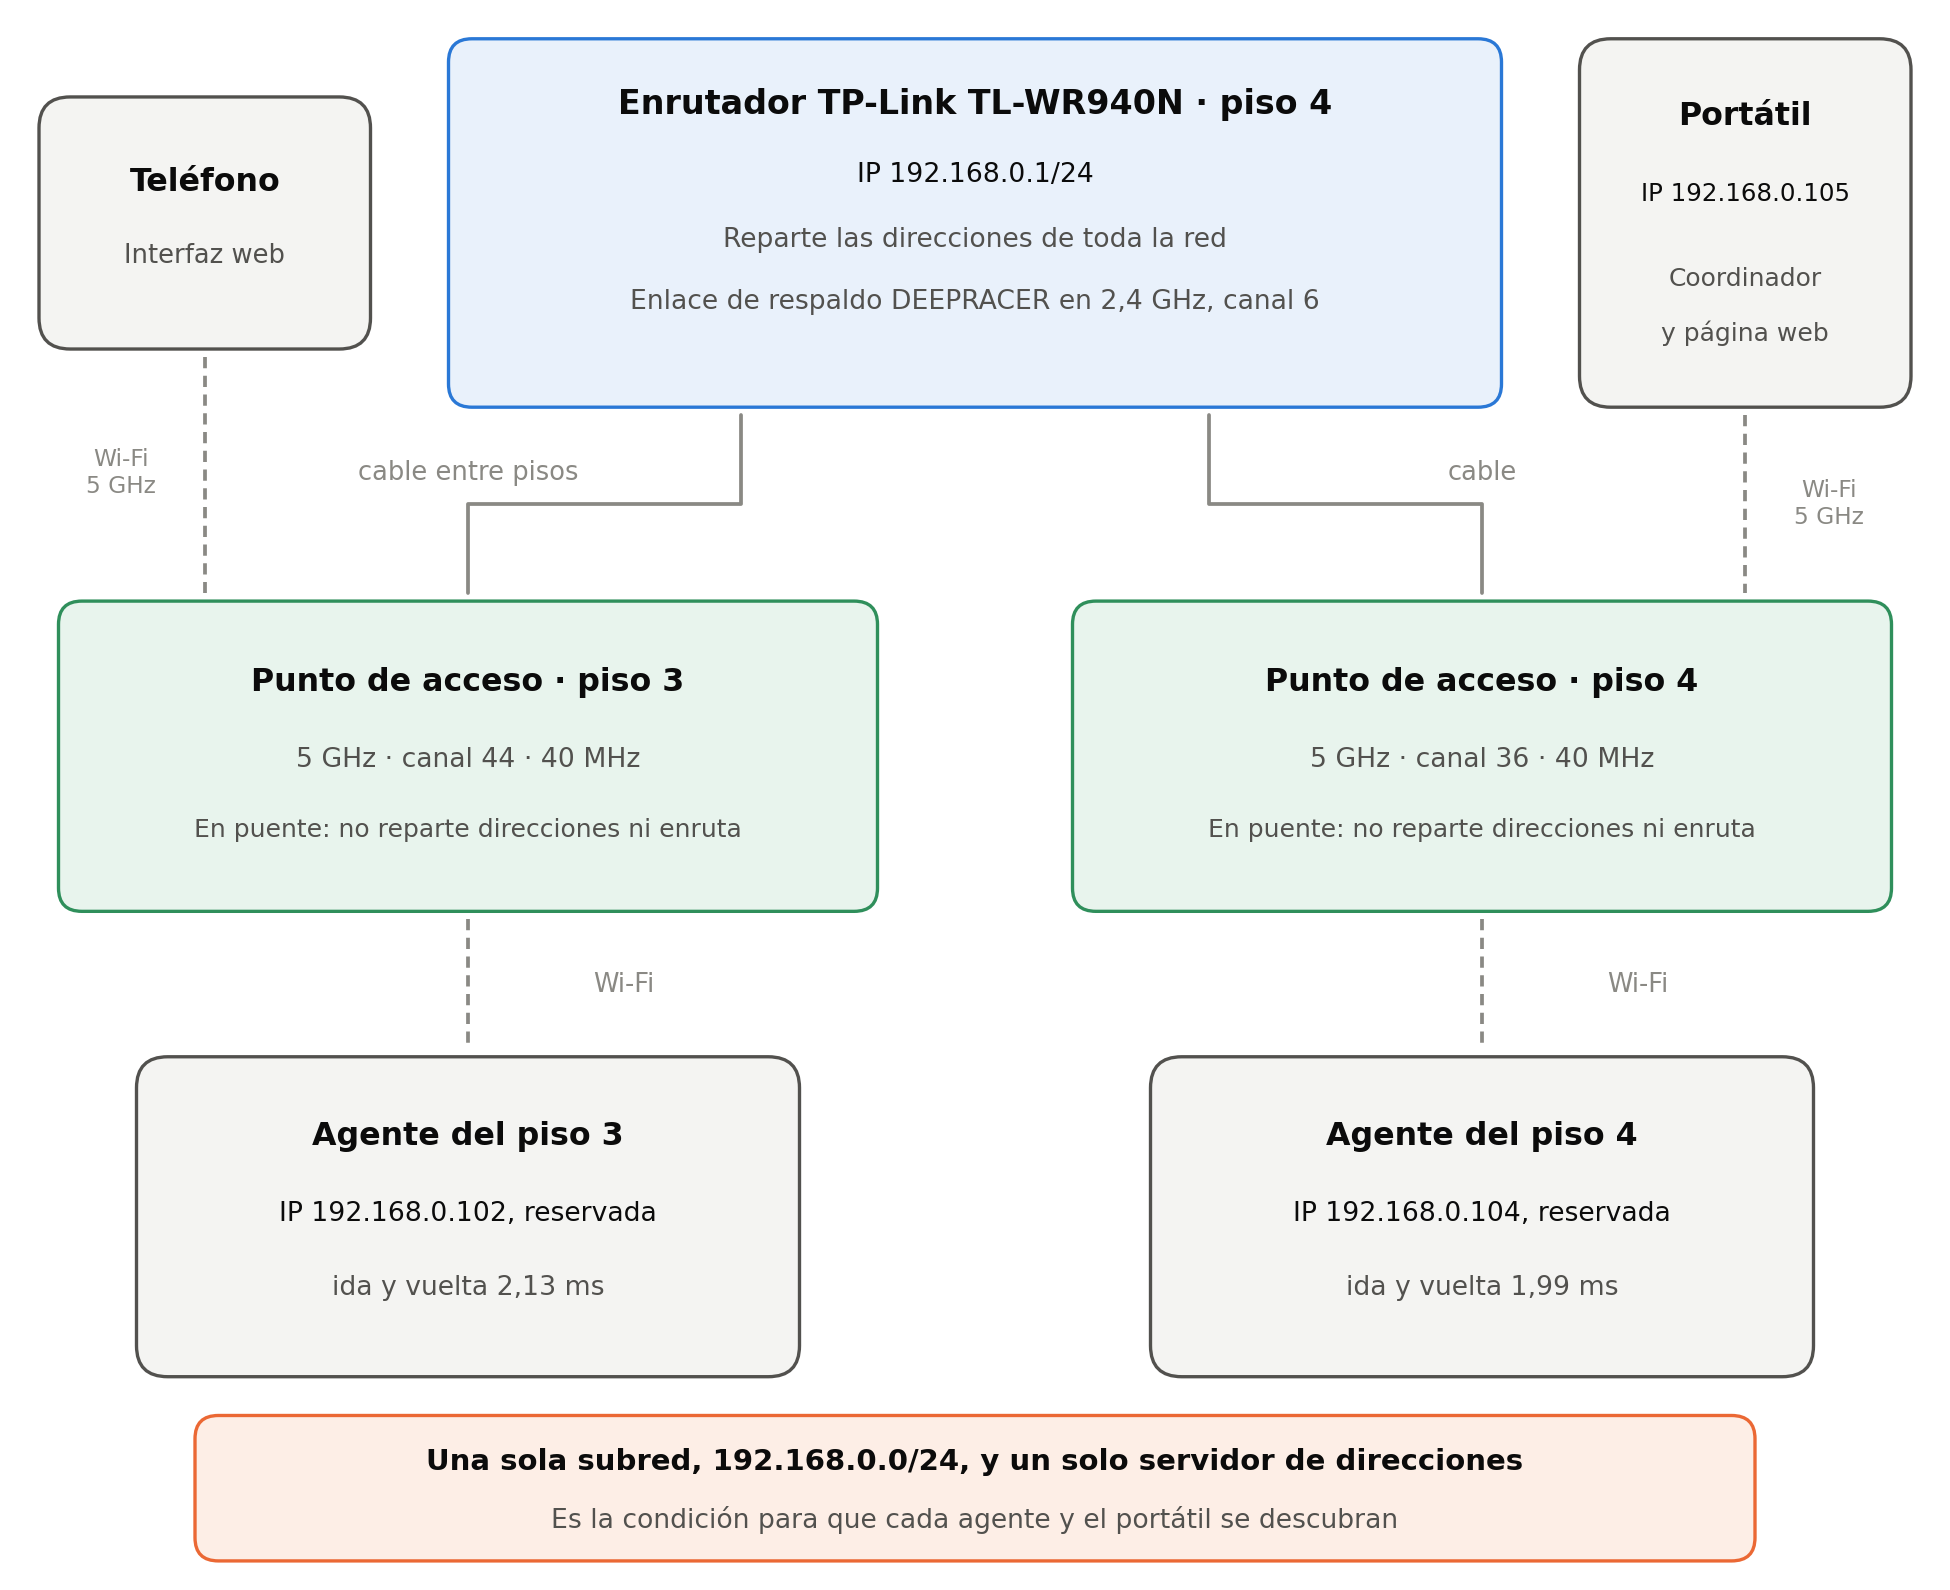
\includegraphics[width=0.84\textwidth]{imagenes/red_topologia.png}
  \caption{Montaje físico de la red en los pisos 3 y 4 del edificio Catalayud, con las direcciones IP y MAC de los equipos.}
  \label{fig:red-topologia}
\end{figure}

El problema de mayor efecto estuvo en cuántos procesos se anunciaban por el enlace. En ROS~2 cada proceso se anuncia periódicamente a todos los demás y mantiene el estado de cada uno, con lo que ese trabajo crece aproximadamente con el cuadrado del número de participantes. Con un agente había del orden de veinte y su tarjeta trabajaba entre el 52 y el 63~\% de capacidad, mientras que al encender el segundo pasaron a ser del orden de cuarenta y la tarjeta subió al 95~\%, con Nav2 sin alcanzar a arrancar. El tráfico, del orden de 2000 paquetes por segundo, era una fracción despreciable del enlace, y la navegación gastaba menos: el aumento estaba en los procesos que atienden la red, y el límite fue el costo de procesamiento del descubrimiento.

\begin{table}[H]
  \centering\footnotesize\setstretch{1.0}
  \caption{Direcciones lógicas y físicas de los equipos de la red en los pisos 3 y 4 del edificio Catalayud.}
  \label{tab:direcciones-red}
  \begin{tabular}{@{}>{\raggedright\arraybackslash}p{0.23\textwidth}>{\raggedright\arraybackslash}p{0.27\textwidth}>{\raggedright\arraybackslash}p{0.22\textwidth}>{\raggedright\arraybackslash}p{0.2\textwidth}@{}}
    \toprule
    \textbf{Equipo} & \textbf{Conexión} & \textbf{Dirección IP} & \textbf{Dirección MAC} \\ \midrule
    Enrutador TP-Link \mbox{TL-WR940N} & En el piso~4; cable a cada punto de acceso y red de respaldo a 2,4~GHz & \texttt{192.168.0.1/24}, fija & \texttt{60:32:B1:77:FB:CC} \\ \addlinespace
    Punto de acceso del piso~3 & Cable entre pisos al enrutador; 5~GHz, canal~44 & --- & \texttt{8C:5F:AD:37:AA:46} \\ \addlinespace
    Punto de acceso del piso~4 & Cable al enrutador, en el mismo piso; 5~GHz, canal~36 & --- & \texttt{8C:5F:AD:37:D2:16} \\ \addlinespace
    Agente del piso~3 & Wi-Fi al punto de acceso de su piso & \texttt{192.168.0.102}, reservada por su MAC & \texttt{80:91:33:ED:8C:F3} \\ \addlinespace
    Agente del piso~4 & Wi-Fi al punto de acceso de su piso & \texttt{192.168.0.104}, reservada por su MAC & \texttt{80:91:33:F3:E6:AB} \\ \addlinespace
    Portátil & Wi-Fi al punto de acceso de su piso, en 5~GHz; la red de 2,4~GHz queda de respaldo & \texttt{192.168.0.105}, asignada por el enrutador & \texttt{D8:80:83:5E:C1:D7} \\ \bottomrule
  \end{tabular}
\end{table}

Restringir el descubrimiento al interior de cada tarjeta bajó el tráfico, pero dejó al coordinador sin ver la navegación de un agente, debido a que el middleware, con pares conocidos, solo anuncia los primeros participantes de cada máquina. La solución fue cambiar dónde vive el coordinador en vez de cómo se anuncian los procesos: el coordinador y el grabador pasaron al portátil, que quedó como único interlocutor conocido de cada agente. Los agentes no se ven entre sí, lo que coincide con el diseño, en el que nunca se comunican directamente, y el sistema completo volvió a entre el 68 y el 74~\% de la tarjeta.

Las cotas del requisito, una mediana de 100~ms y un percentil 95 de 250~ms sin pérdidas, se fijaron antes de medir, a partir de los 2~Hz a los que cada agente publica su estado. Entre los dos agentes, en la misma sala y sobre 600 mensajes, la mediana fue de 5,99~ms y el percentil 95 de 11,12~ms, sin pérdidas, más de un orden de magnitud por debajo de las cotas. Con paquetes de red, entre los dos agentes en el mismo piso y con dos puntos de acceso, la ida y vuelta fue de 3,75~ms en promedio. En el montaje definitivo, con cada agente en el punto de acceso de su piso del edificio Catalayud, fue de 2,13 y 1,99~ms contra el enrutador, sin pérdidas ni duplicados. Por lo tanto, la red no limita el desempeño del sistema, cuyos límites están en la plataforma.

\subsection{Integración de los módulos}
\label{sec:integracion}
\label{sec:simulacion}
\label{sec:sim-a-vehiculos}

La integración partió de una revisión de la base de trabajo. El espacio donde se compilaba el código era una copia del repositorio del fabricante, sin enlace al del proyecto, así que los ajustes del mapeo hechos hasta entonces nunca se habían ejecutado; se enlazó al repositorio del proyecto, y sobre él se fijó el contrato de interfaces.

Los escenarios de los pisos 2 y 3 del edificio Gregorio se montaron en Gazebo~11 con ROS~2 Humble, cuyo enlace con el simulador aplica a todos los complementos el espacio de nombres del primer modelo cargado, lo que impidió tener dos agentes en un mismo proceso. Con los dos pisos en un mismo mundo, además, el láser simulado, de 10~m de alcance, veía paredes del otro piso en 61 de 1701 posiciones muestreadas, justo donde arranca el primer agente y donde está su punto de transferencia. Por esas razones cada piso es un mundo distinto, con su propio proceso de simulación, y los dos agentes comparten un dominio de comunicaciones, separados por espacio de nombres. La figura~\ref{fig:sim-relevo} muestra una misión con relevo entre los dos procesos, completada en 100,1~s.

El mapa de navegación de esos pisos se calculó de la geometría del modelo y es exacto en simulación. Otro mapa construido con SLAM cubría el 35,5~\% del largo del pasillo, medía 15,0~m de ancho frente a los 5,3~m del mundo simulado, y 2688 de sus 3618 celdas ocupadas, el 74~\%, no tenían ninguna pared detrás. Como un mapa de ocupación es un corte horizontal, el del piso superior resultó idéntico.

Como los mundos simulados de los pisos 3 y 4 del edificio Catalayud salen del mismo levantamiento que sus mapas, el sistema también puede ejecutarse en simulación en esos pisos, con un proceso de Gazebo por piso (figura~\ref{fig:sim-catalayud}), los mismos mapas, los mismos destinos y la misma página. De trece misiones, diez se completaron, tres se cancelaron a propósito y ninguna falló, con llegadas entre 0,067 y 0,206~m. Funcionaron además dos partes que hasta entonces solo se habían usado con los agentes físicos, la maniobra de media vuelta y la verificación de la llegada con la posición del agente en el mapa. Fue una comprobación de funcionamiento, sin el protocolo de la campaña, que no entra en sus resultados, y la simulación sigue sin reproducir la odometría real, la respuesta de la tracción y la red entre pisos.

Al llevar el sistema a los agentes físicos se mantuvo su estructura: un coordinador, un agente por piso, el relevo en la escalera y las reglas del contrato. También se mantuvo el código del coordinador, del planificador, de los mensajes y de la página, que compila sin cambios en las dos distribuciones de ROS~2 y completó una misión en cada una. La integración con los agentes físicos se comprobó con seis pruebas de verificación sucesivas, cada una con un criterio escrito antes de ejecutarla y con lo que significa no superarla (tabla~\ref{tab:pruebas-verificacion}).

\begin{figure}[H]
  \centering
  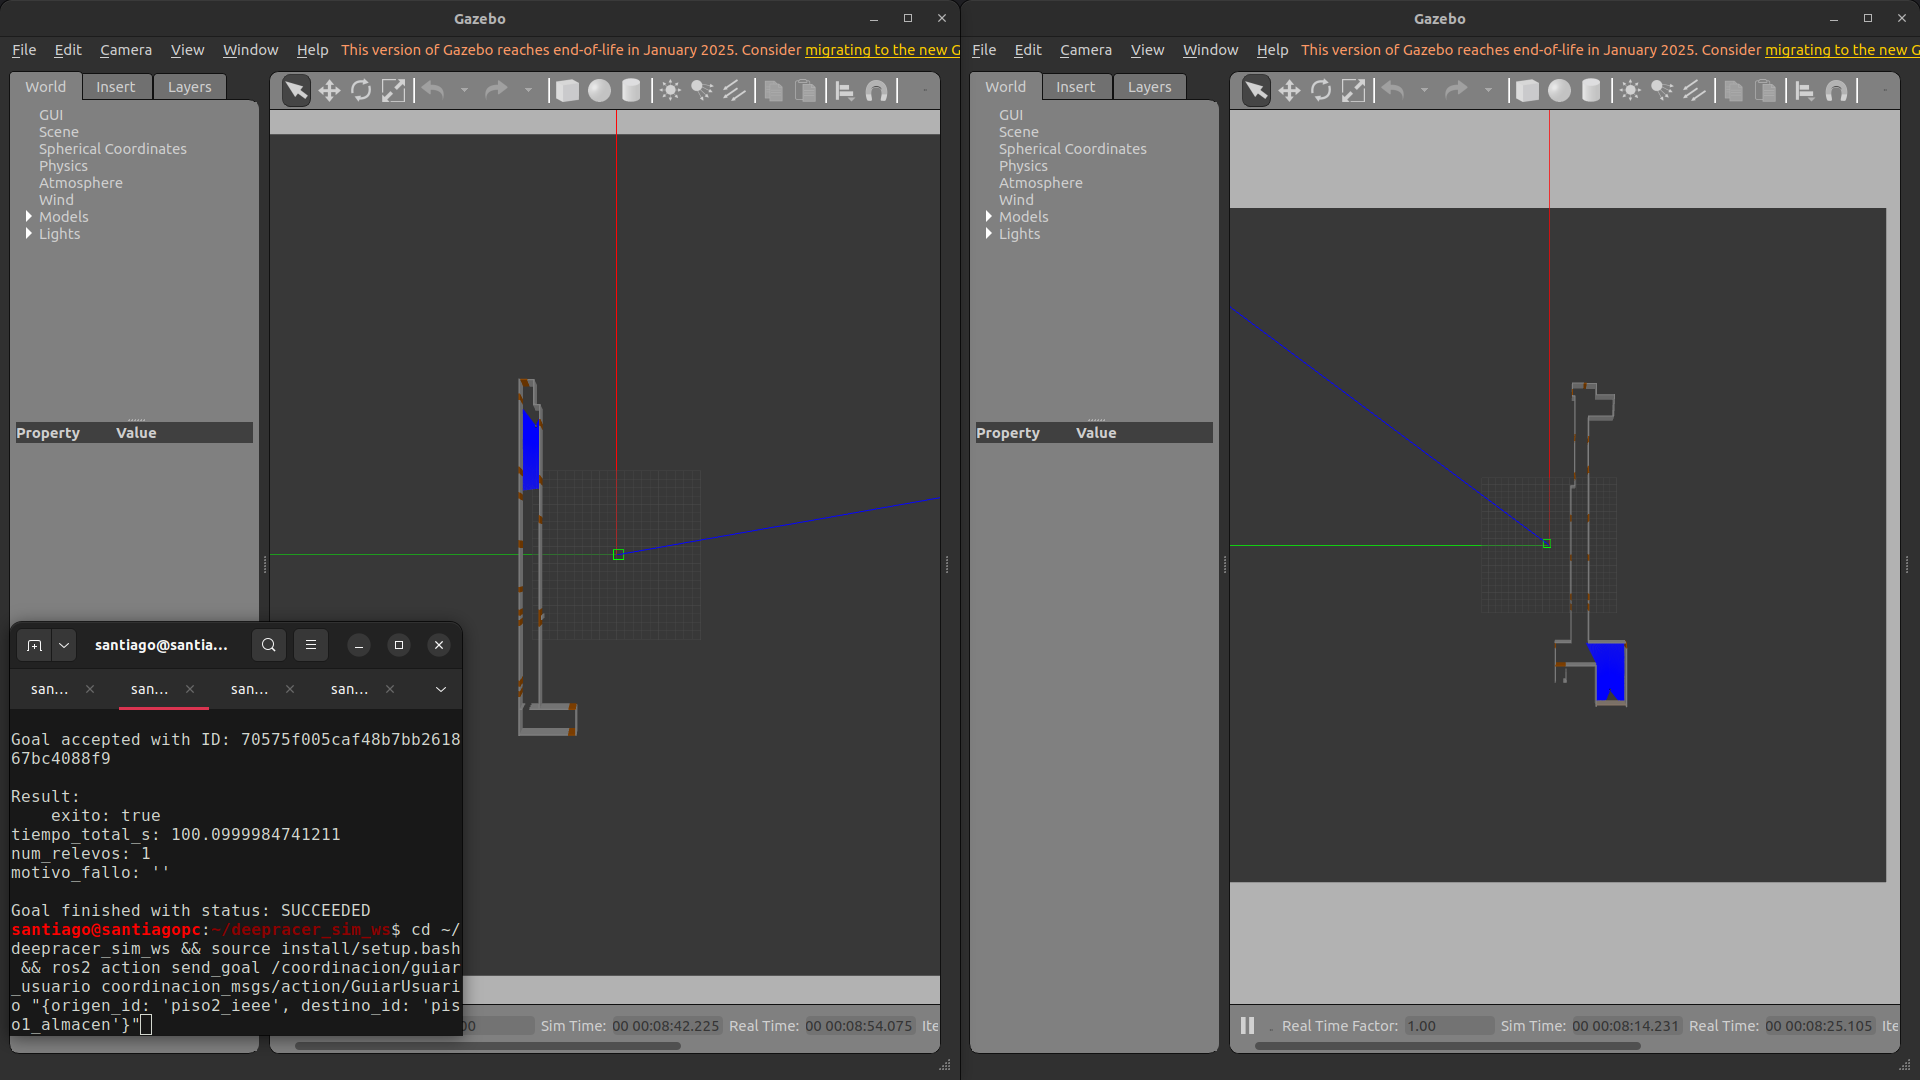
\includegraphics[width=0.66\textwidth]{imagenes/simulacion_relevo_dos_procesos.png}
  \caption{Misión con relevo en simulación, con un proceso de Gazebo por piso.}
  \label{fig:sim-relevo}
\end{figure}

\begin{figure}[H]
  \centering
  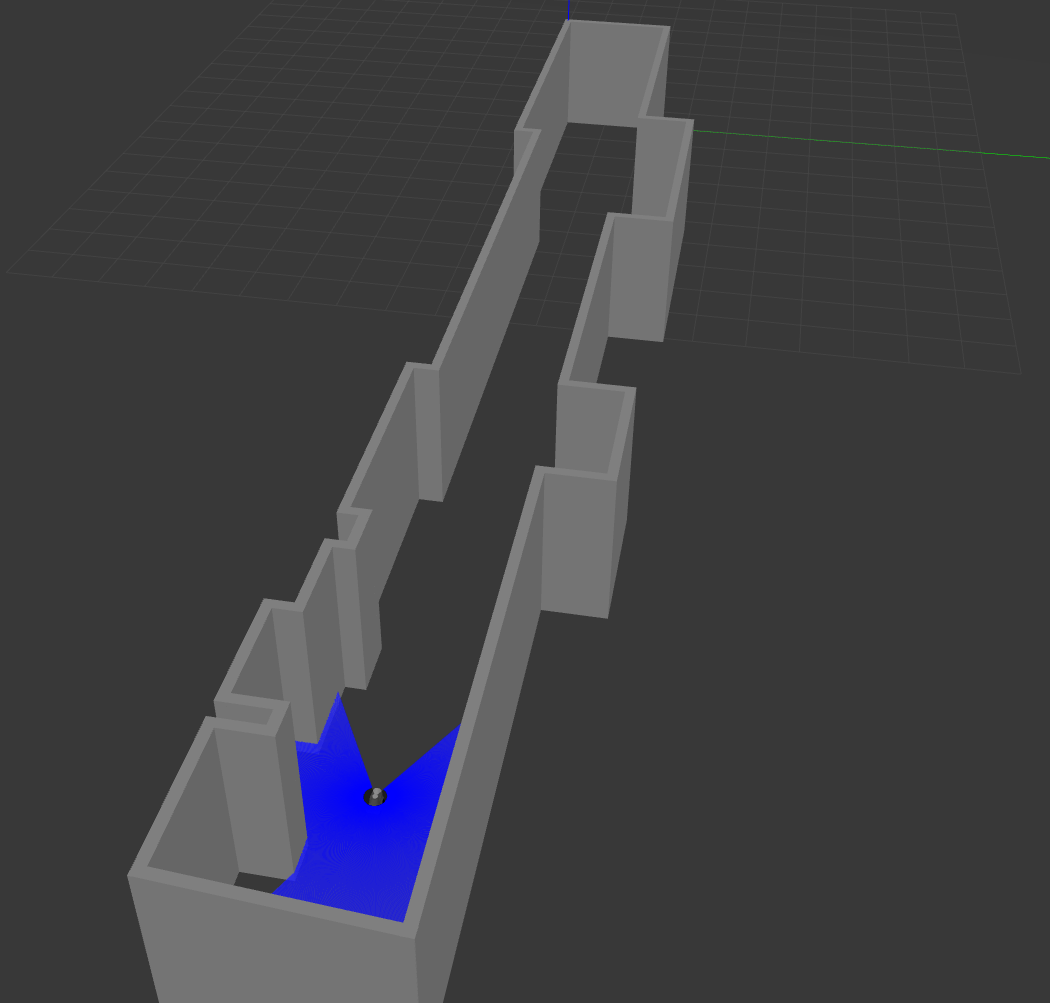
\includegraphics[width=0.49\textwidth]{imagenes/simulacion_catalayud_piso3.png}\hfill
  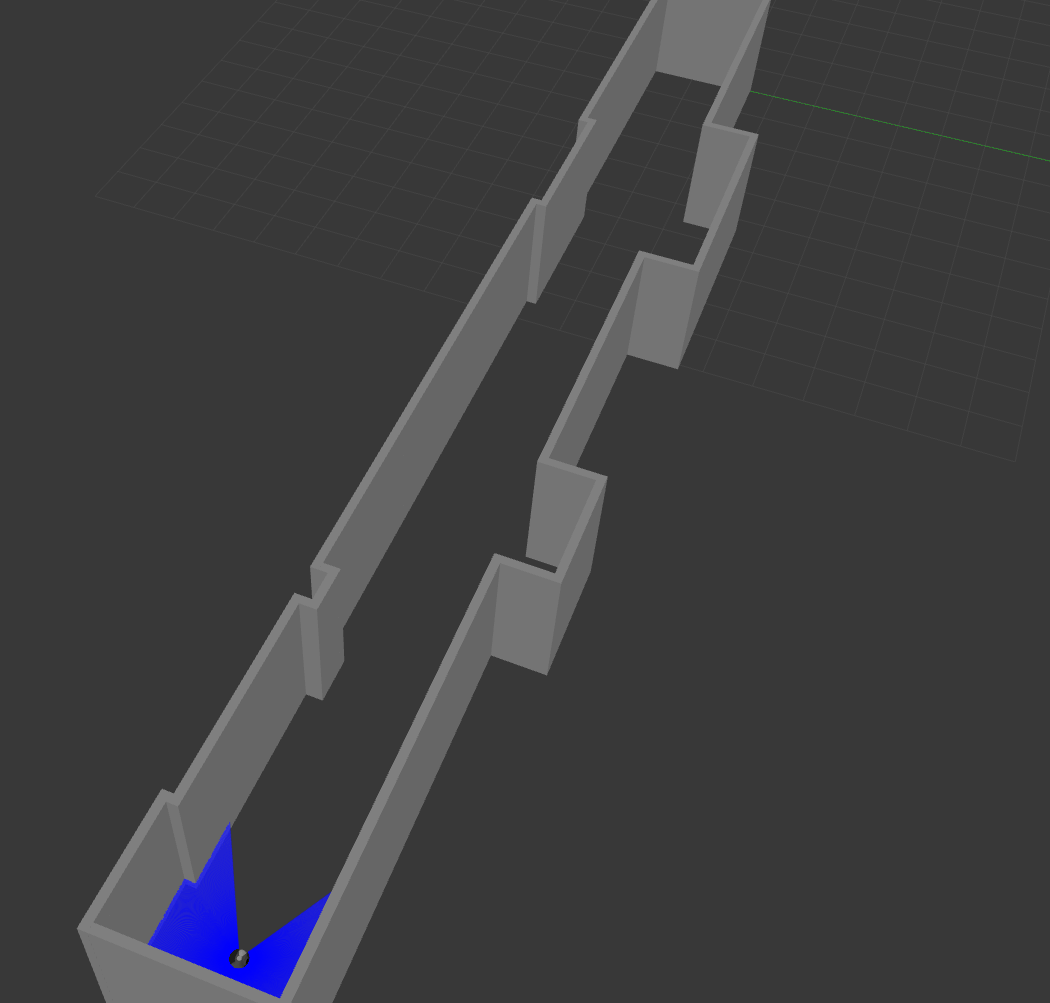
\includegraphics[width=0.49\textwidth]{imagenes/simulacion_catalayud_piso4.png}
  \caption{Pisos 3 (izquierda) y 4 (derecha) del edificio Catalayud en simulación.}
  \label{fig:sim-catalayud}
\end{figure}

\label{sec:pruebas-verificacion}
\begin{table}[H]
  \centering\footnotesize\setstretch{1.0}
  \caption{Pruebas de verificación de la demostración física, todas superadas al cerrar la toma de datos.}
  \label{tab:pruebas-verificacion}
  \begin{tabular}{@{}>{\raggedright\arraybackslash}p{0.3\textwidth}>{\raggedright\arraybackslash}p{0.64\textwidth}@{}}
    \toprule
    \textbf{Prueba} & \textbf{Criterio} \\ \midrule
    Actuación & El agente responde a las órdenes de dirección y tracción \\
    Odometría & Error de 10~\% o menos sobre un recorrido conocido de 5~m o más \\
    Navegación de un agente & Un agente llega de un punto a otro con Nav2, con la llegada verificada \\
    Dos agentes en la misma red & Los dos agentes y el coordinador coexisten sin conflicto de nombres \\
    Misión con relevo & Una misión con relevo sobre los dos agentes, con su registro \\
    Campaña con los agentes físicos & Entre 5 y 10 repeticiones del protocolo con su registro \\ \bottomrule
  \end{tabular}
\end{table}

Lo que cambió fue la implementación de los bloques. La tabla~\ref{tab:sim-vehiculos} reúne cada cambio con su causa, y la figura~\ref{fig:arquitectura-vehiculos} muestra el sistema como funcionó en la campaña con los agentes físicos.

\begin{table}[H]
  \centering\footnotesize\setstretch{1.0}
  \caption{Cambios en la implementación al pasar de la simulación a los agentes físicos.}
  \label{tab:sim-vehiculos}
  \begin{tabular}{@{}>{\raggedright\arraybackslash}p{0.13\textwidth}>{\raggedright\arraybackslash}p{0.205\textwidth}>{\raggedright\arraybackslash}p{0.285\textwidth}>{\raggedright\arraybackslash}p{0.30\textwidth}@{}}
    \toprule
    \textbf{Parte} & \textbf{En simulación} & \textbf{En los agentes físicos} & \textbf{Causa} \\ \midrule
    Distribución de ROS~2 & Humble en todos los componentes & Jazzy en los agentes y en el coordinador, en un contenedor del portátil; Humble en la página y en rosbridge & El software de la tarjeta solo existe para Ubuntu 24.04 con Jazzy, la simulación no existe en Jazzy, y la acción de navegación de Jazzy no es compatible con la de Humble \\ \addlinespace
    Coordinador & En el portátil, junto a los dos simuladores & En el portátil, después de un intento en uno de los agentes & Con el coordinador y el grabador en una tarjeta y las dos navegaciones encendidas, la carga subió de 6 a entre 17 y 33 y Nav2 no arrancaba \\ \addlinespace
    Comunicación & Un computador y un dominio de comunicaciones; un espacio de nombres por agente & Red inalámbrica con un punto de acceso de 5~GHz por piso; una partición por agente y topología en estrella hacia el portátil & Los tópicos del fabricante no llevan espacio de nombres, y los procesos de las dos cadenas, anunciándose por la red, saturaban las tarjetas \\ \addlinespace
    Locomoción & Complemento Ackermann de Gazebo & Puente de la orden de velocidad a los servos, con una escala por agente & La tracción real tiene banda muerta y funciona en lazo abierto \\ \addlinespace
    Sensado & Láser simulado de 10~m de alcance & RPLIDAR A1M8 y la unidad inercial de la tarjeta; cámaras apagadas & Las cámaras no se usan y cargaban la tarjeta \\ \addlinespace
    Odometría & La del simulador & La del láser, combinada con la unidad inercial mediante un filtro & El agente no tiene codificadores en las ruedas, y con el láser solo el rumbo derivaba 5,9$^\circ$ por minuto \\ \addlinespace
    Mapa & Calculado del mundo simulado & Derivado de la planta medida con flexómetro & El mapeo con SLAM a bordo no dio un mapa utilizable en ningún pasillo \\ \addlinespace
    Escenario & Pisos 2 y 3 del edificio Gregorio & Pisos 3 y 4 del edificio Catalayud, levantados con flexómetro & Tránsito de personas, mundo simulado mal medido y pasillos uniformes en Gregorio \\ \addlinespace
    Llegada & Tolerancia de 0,25~m & Tolerancia de 0,5~m, verificada con la pose del agente 1,5~s después de que Nav2 da la meta por alcanzada & Por la banda muerta, el agente no alcanza la precisión de la simulación, y sigue rodando cuando Nav2 declara la llegada \\ \addlinespace
    Media vuelta & La planifica Nav2, con marcha atrás & Maniobra propia del agente, vigilada con el láser y el mapa & En la salida del piso 4 de Catalayud, de 2,5~m de ancho, la media vuelta de Nav2 abortó contra la pared \\ \bottomrule
  \end{tabular}
\end{table}

\begin{figure}[H]
  \centering
  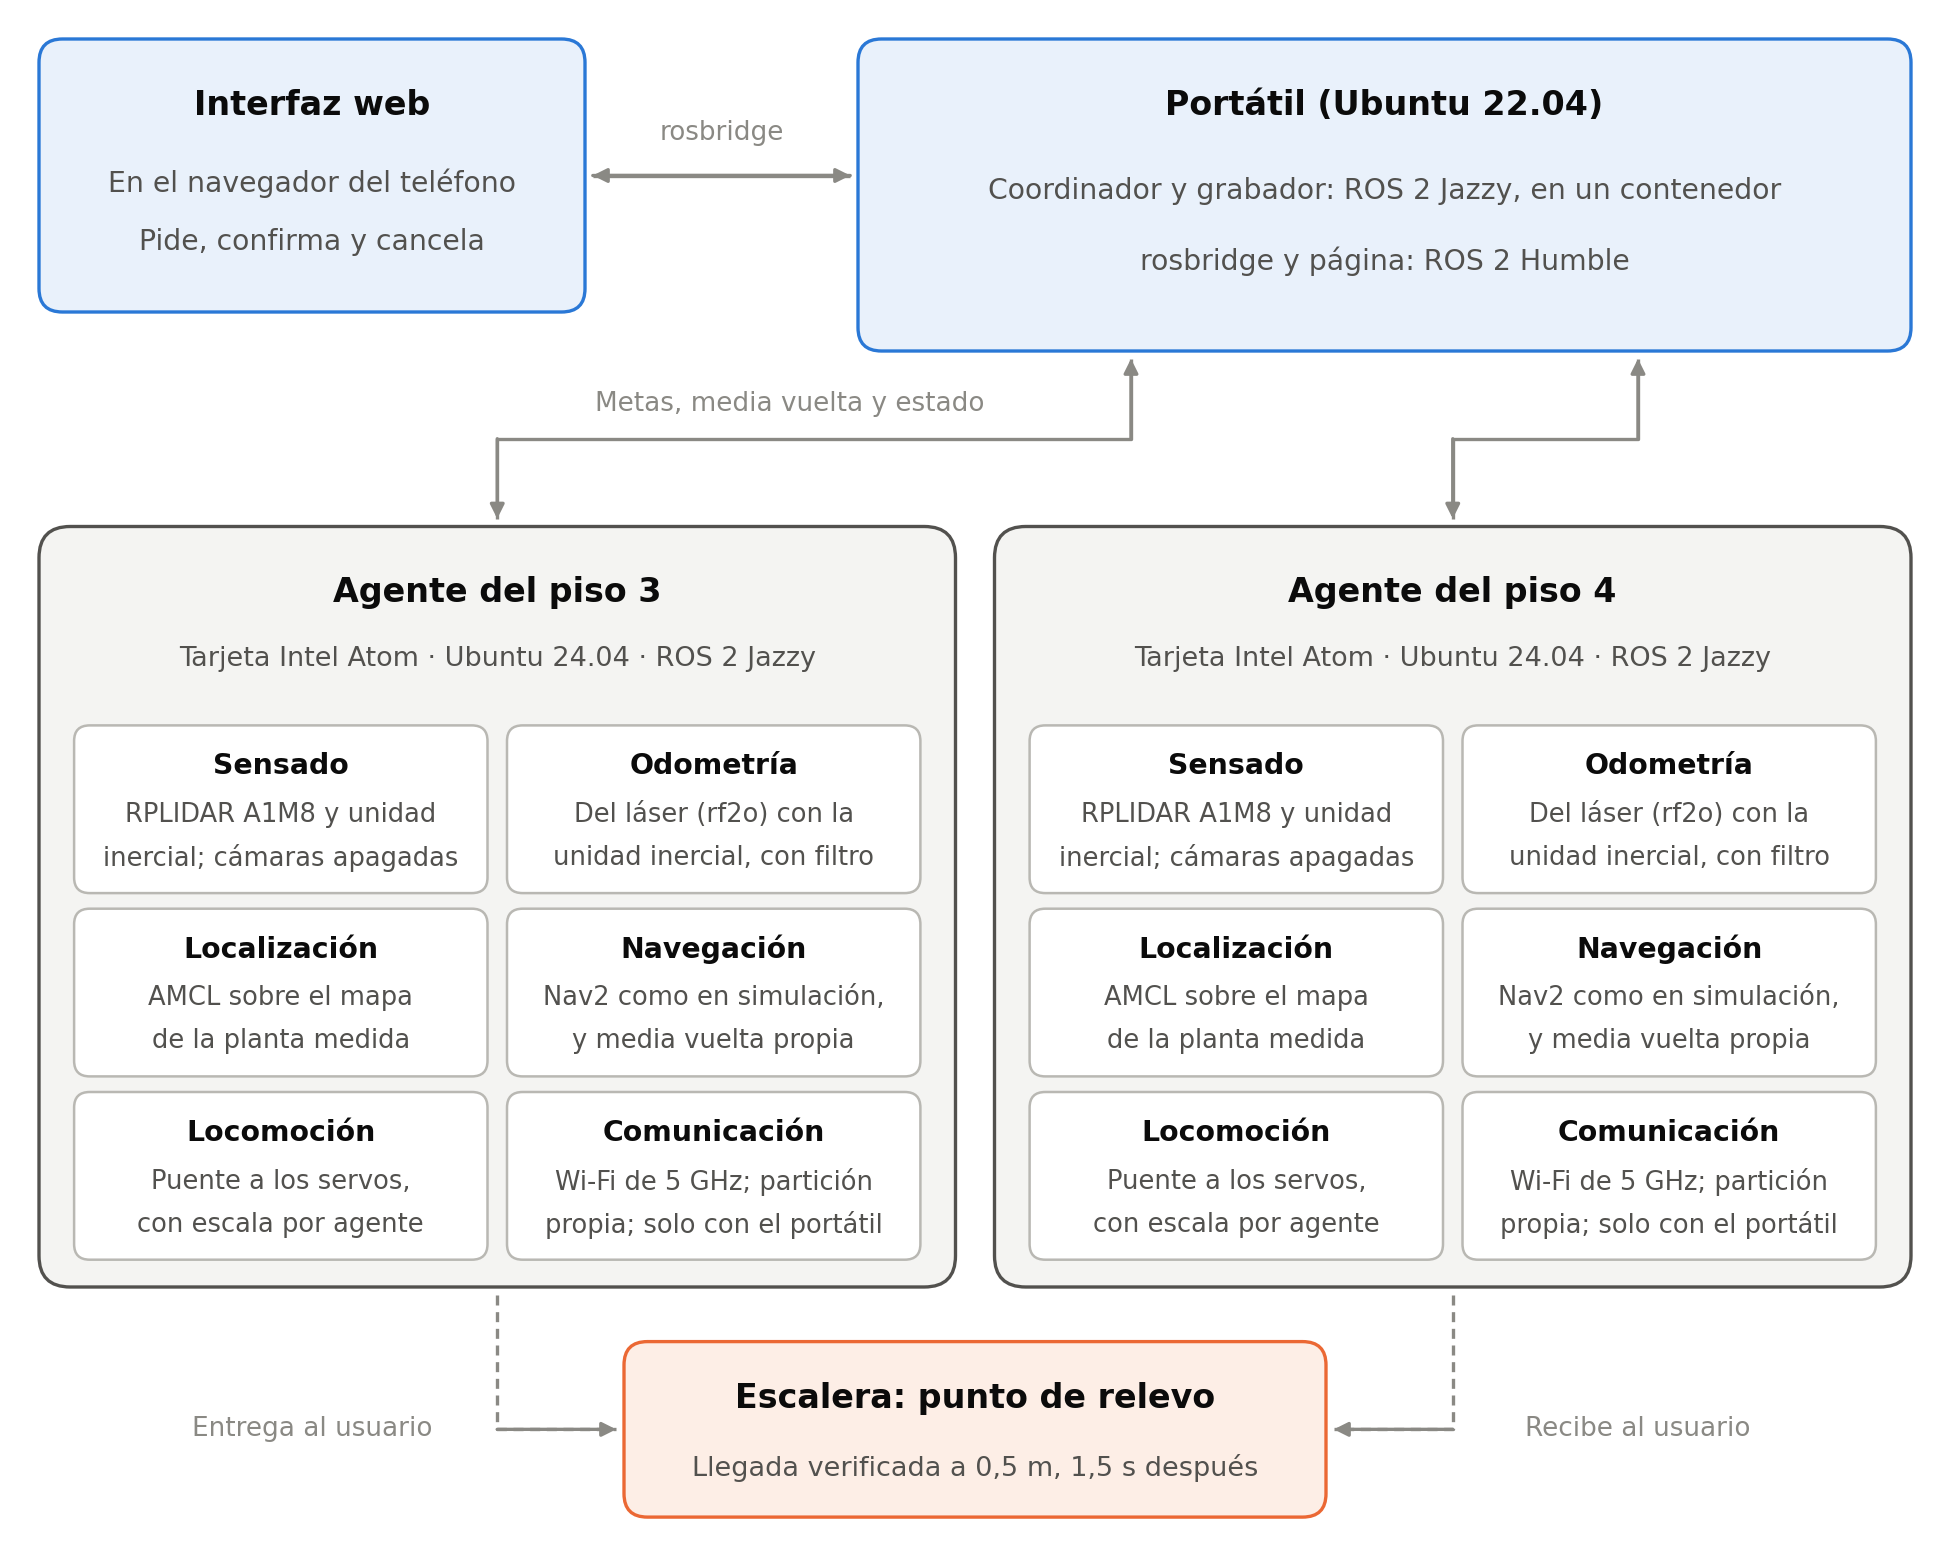
\includegraphics[width=0.86\textwidth]{imagenes/arquitectura_vehiculos.png}
  \caption{Arquitectura del sistema en la campaña con los agentes físicos.}
  \label{fig:arquitectura-vehiculos}
\end{figure}

% =====================================================================
\section{Tercer objetivo específico: interfaz móvil}
\label{sec:oe3}

El objetivo pide una interfaz móvil basada en la selección de localizaciones de origen y destino, y se cumplió con una página web que se abre en el navegador del teléfono, porque un usuario ocasional no va a instalar nada para preguntar por un salón. La página funciona sin salida a internet, puesto que la red del edificio puede no tenerla, y no usa bibliotecas ni recursos externos: son un archivo HTML, una hoja de estilo y dos programas en JavaScript, que sirve el propio portátil en el puerto 8000. El primer programa es un cliente propio del protocolo del puente \textit{rosbridge}, en el puerto 9090, y el segundo es la lógica de la página, que recibe el catálogo de puntos al conectarse y el estado de la misión una vez por segundo, pide y cancela con la acción de guiado y publica la confirmación de cambio de piso. Como el puente no tiene autenticación, el firewall del portátil solo admite conexiones desde la red de los agentes.

\subsection{Selección de origen y destino}

El usuario elige el origen en una lista y el destino en un catálogo con búsqueda por nombre, donde cada destino muestra su piso y, si queda en el otro piso, la marca «con relevo» (figura~\ref{fig:hri}, izquierda). Durante la misión, la página muestra un título calculado a partir de la etapa, el texto que redacta el coordinador, el agente que está guiando, hacia dónde va, el destino final y la distancia restante, y una franja de cinco pasos (preparando, tramo 1, relevo, tramo 2 y fin) marca el paso actual (figura~\ref{fig:hri}, centro).

La interfaz se verificó contra el coordinador real: el catálogo, una misión con sus etapas, el texto del coordinador mostrado literal y el botón que se reactiva al terminar. También se operó una misión completa con relevo desde un teléfono conectado a la red de los agentes, sin tocar el computador.

\begin{figure}[H]
  \centering
  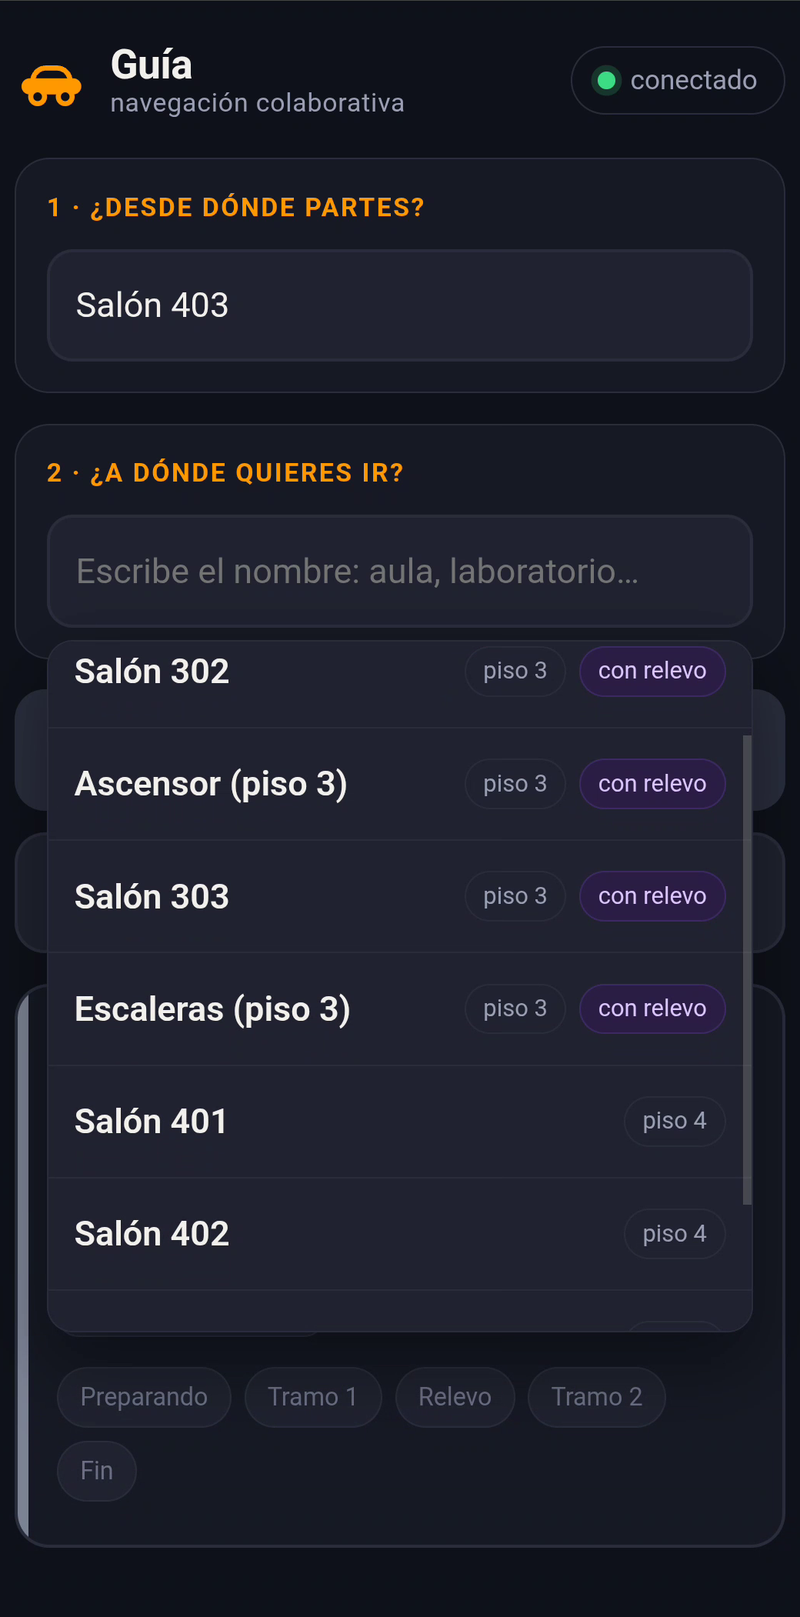
\includegraphics[height=7.6cm]{imagenes/hri_catalogo.png}\hfill
  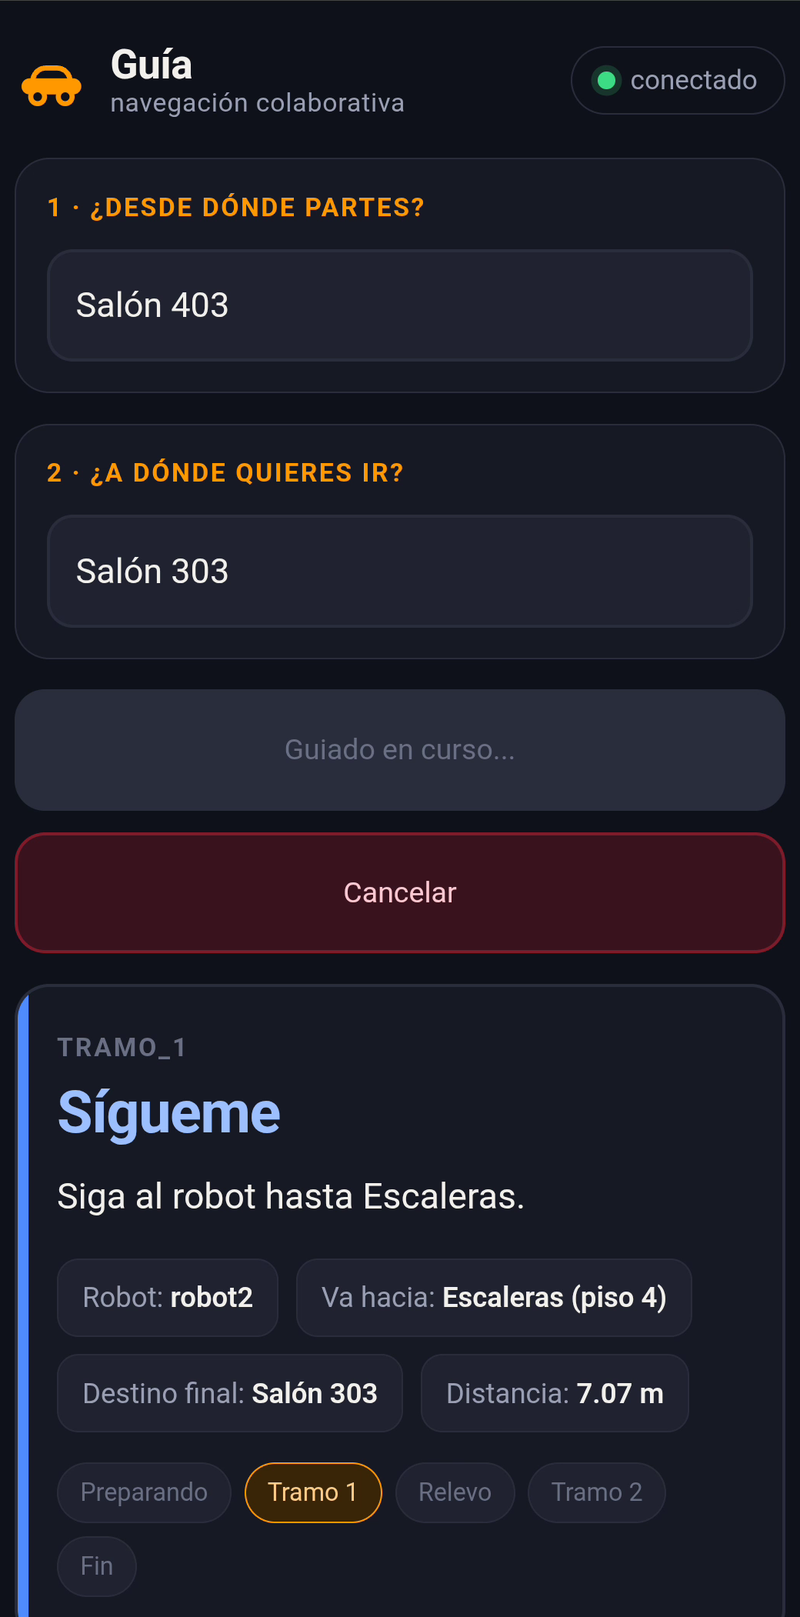
\includegraphics[height=7.6cm]{imagenes/hri_seguimiento.png}\hfill
  \begin{minipage}[b]{3.35cm}
    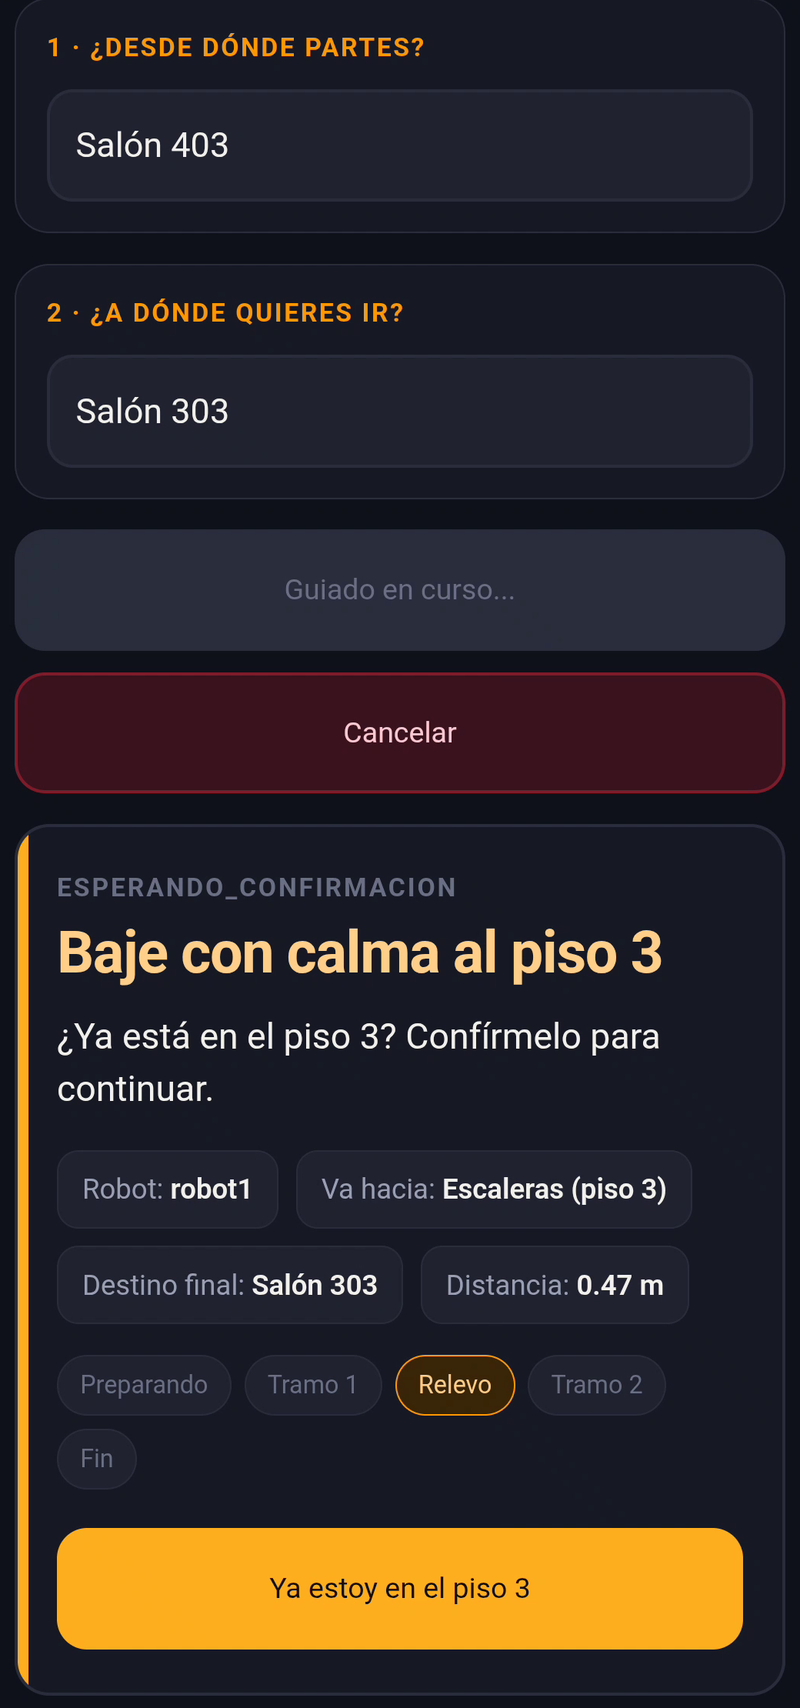
\includegraphics[trim=0 0 0 818,clip,width=\linewidth]{imagenes/hri_confirmacion_piso.png}\\[0.2cm]
    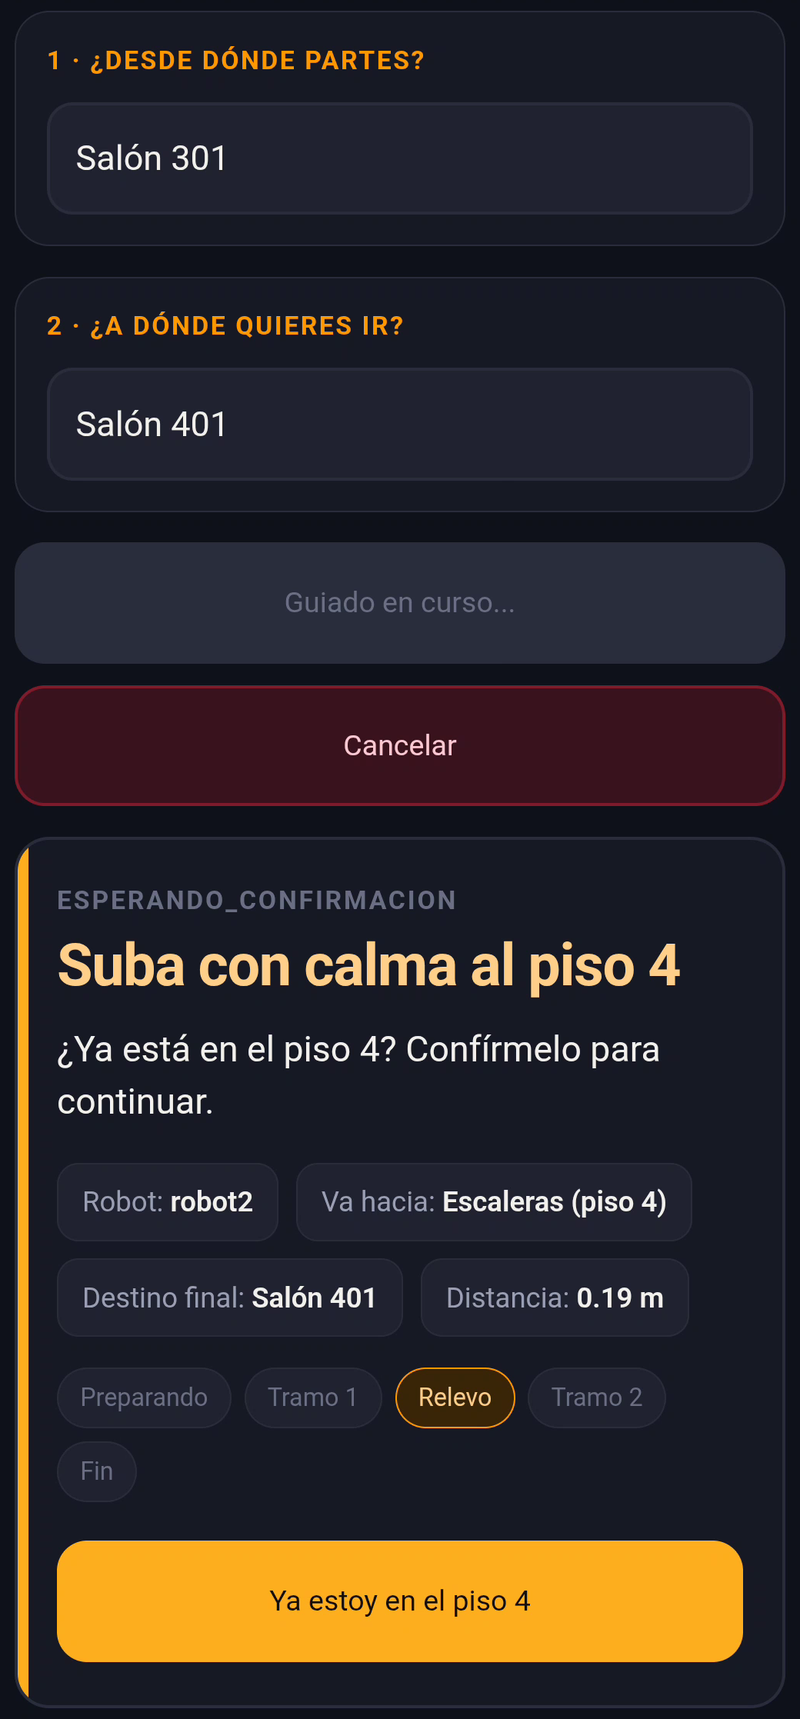
\includegraphics[trim=0 0 0 832,clip,width=\linewidth]{imagenes/hri_confirmacion_subida.png}
  \end{minipage}
  \caption{Interfaz web en el teléfono durante las pruebas del 23 de octubre (anexo A, video 8): catálogo de destinos (izquierda), primer tramo de una misión (centro) y espera de confirmación al bajar y al subir (derecha).}
  \label{fig:hri}
\end{figure}

\subsection{Confirmación de cambio de piso}

En una misión entre pisos, el segundo agente llega a su escalera y no puede saber si el usuario ya cambió de piso. Sin una pausa explícita, la misión podía darse por completada con el usuario todavía en el piso equivocado, y la instrumentación lo habría registrado como éxito. Por esa razón, cuando el segundo agente llega a su punto de transferencia, el coordinador pasa a la etapa de espera y la página muestra un botón para confirmar el cambio de piso, que solo existe en esa etapa (figura~\ref{fig:hri}, derecha). A los 60~s sin confirmación aparece un aviso, y a los 120~s la misión termina como fallida. Los plazos se cuentan desde que llega el agente, para que un agente lento no le consuma tiempo al usuario, y se miden con el reloj del sistema, sin depender del de la simulación. Si el usuario confirma antes de que el agente llegue, la confirmación se retiene y se aplica al llegar.

Se verificó en simulación con una ejecución por camino: confirmar a los pocos segundos termina la misión con éxito, confirmar pasados los 60~s hace aparecer el aviso en el teléfono, y no confirmar deja la misión fallida a los 120~s, con el motivo redactado.


\subsection{Cancelación}

El botón de cancelar no tenía efecto en la primera versión, ya que el servidor de acción del coordinador no registraba la función que responde a la cancelación y ROS~2 rechaza por omisión, sin informar, toda cancelación que no tenga esa función. Al corregirlo se añadió el comportamiento que faltaba: la misión pasa por la etapa de cancelación, el agente activo regresa al punto de transferencia de su piso y la misión cierra como fallida con un texto que lo dice. En simulación, con una ejecución cancelada y una de control, el agente quedó a 0,121~m de su punto de regreso.

Con los agentes físicos se cancelaron seis misiones en los pisos 3 y 4 del edificio Catalayud, al menos una en cada etapa (anexo A, video 8), y en las seis el agente volvió a su escalera, a entre 0,07 y 0,34~m de su punto. En esas pruebas apareció un defecto que la simulación no podía mostrar, pues la media vuelta propia se añadió después. Nav2 conserva durante un tiempo las metas terminadas, y mientras tenía una cancelada en su lista, el agente se declaraba en error y rechazaba la media vuelta, y Nav2 intentaba girar por su cuenta en el pasillo y oscilaba. Se corrigió haciendo que la media vuelta solo espere a que no haya una meta en curso: antes de la corrección se rechazaron ocho de quince medias vueltas, y después ninguna de diez.

\subsection{Ajustes tras las pruebas con los agentes físicos}
\label{sec:ajustes-campo}

En las pruebas con los agentes físicos aparecieron además defectos de la página. El título de la etapa de confirmación preguntaba siempre «¿Ya subió?», lo que al subir resultaba brusco y al bajar del piso 4 al 3 era falso. Por ello pasó a salir de comparar el piso de origen con el del agente que espera, como «Suba con calma al piso 4» o «Baje con calma al piso 3» (figura~\ref{fig:hri}), y el botón dice «Ya estoy en el piso 4», o el piso que corresponda. Ese cambio se hizo el día de la campaña, antes de ejecutarla, y aun así los teléfonos mostraron la versión anterior, debido a que el servidor no le indicaba al navegador cuándo volver a pedir la página; desde entonces la página se sirve con la indicación de comprobarla cada vez que se abre. Por otra parte, los dos ascensores del edificio Catalayud se llamaban igual en la lista y en una misión se eligió el del piso equivocado, así que los nombres repetidos se muestran con su piso, como «Ascensor (piso 3)» (figura~\ref{fig:hri}, izquierda). Los tres ajustes se verificaron con pruebas automáticas y después con un teléfono y los agentes físicos, en una misión de subida y otra de bajada.

% =====================================================================
\section{Cuarto objetivo específico: evaluación experimental}
\label{sec:protocolo}

La evaluación se hizo con las cuatro métricas que nombra el objetivo: tiempo de respuesta, tiempo de asignación, tasa de éxito y continuidad del servicio entre niveles.

\subsection{Métricas y criterio de éxito}

El protocolo se escribió antes de instrumentar el sistema, porque un protocolo redactado después de ver los datos tiende a acomodarse a lo que salió, por ejemplo eligiendo el umbral que deja fuera las ejecuciones malas. Fija las métricas con su definición operativa, el criterio de éxito, el tamaño de muestra y una lista cerrada de causas de descarte, y cada versión queda fechada en el historial del repositorio.

Una métrica sin un evento de inicio y uno de fin medibles por una máquina no se puede informar, de ahí que la tabla~\ref{tab:metricas} dé los dos eventos de cada una. Todas las marcas salen de un mismo reloj: en simulación, el de la simulación; en los agentes físicos, el del computador que graba.

\begin{table}[H]
  \centering\footnotesize\setstretch{1.0}
  \caption{Definición operativa de las cuatro métricas del anteproyecto.}
  \label{tab:metricas}
  \begin{tabular}{@{}>{\raggedright\arraybackslash}p{0.2\textwidth}>{\raggedright\arraybackslash}p{0.36\textwidth}>{\raggedright\arraybackslash}p{0.36\textwidth}@{}}
    \toprule
    \textbf{Métrica} & \textbf{Inicio} & \textbf{Fin} \\ \midrule
    Tiempo de respuesta & El coordinador acepta la solicitud & Primera de tres muestras seguidas de la odometría del agente asignado con velocidad de al menos 0,02~m/s \\ \addlinespace
    Tiempo de asignación & Primera publicación de la etapa recibida & Primera publicación del primer tramo, con el agente asignado \\ \addlinespace
    Tasa de éxito & \multicolumn{2}{p{0.72\textwidth}}{Proporción de misiones exitosas sobre las ejecuciones válidas} \\ \addlinespace
    Continuidad entre niveles & El primer agente alcanza su punto de transferencia & Primer movimiento del segundo agente \\ \bottomrule
  \end{tabular}
\end{table}

Una misión es exitosa si la pose final del agente, en su odometría, está a 0,25~m o menos del destino declarado en el catálogo (0,5~m en los agentes físicos), si llegó a la etapa completada sin pasar por fallida y, cuando era entre pisos, si hubo un relevo. La regla central del protocolo es que el éxito se mide contra la odometría del agente, sin tomar por válido el resultado que devuelve Nav2. Una navegación puede terminar en éxito y haber dejado al agente lejos del destino: en las primeras pruebas en simulación, una de tres metas devolvió éxito con el agente a 0,296~m. Aceptar ese resultado sería dejar que el sistema se evalúe a sí mismo.

El tiempo de asignación resultó menor que el paso de 100~ms del reloj de la simulación, así que se informa como una cota por misión y se caracterizó aparte, en un banco de pruebas con el reloj del sistema. La continuidad se definió primero como una condición binaria, que resultó no poder fallar, y se reemplazó por el intervalo del relevo, una magnitud que sí varía.

\subsection{Campañas de evaluación}

La campaña en simulación, en los pisos 2 y 3 del edificio Gregorio (anexo A, video 6), tiene treinta misiones en dos grupos de quince. En las de un mismo piso no hay relevo y sirven de comparación; en las de dos pisos hay un relevo, y son las que responden la pregunta de investigación.

Los pares de origen y destino salen de un sorteo, pues con pares elegidos a mano se corre el riesgo de probar justo los recorridos que funcionan. Se sortean entre los puntos del catálogo menos los dos puntos de transferencia, catorce en el piso 2 y quince en el piso 3, que dan 392 pares posibles dentro de un mismo piso y 420 entre pisos, y ningún par se repite. La semilla del sorteo es la fecha en que se hace, escrita como año, mes y día, y el listado se guarda en el repositorio antes de la primera ejecución, de manera que nadie puede probar semillas hasta obtener un sorteo conveniente.

Las diez primeras misiones salieron de un sorteo con la semilla 20260822 en el que todas las misiones entre pisos subían del piso 2 al 3 y todas las de un solo piso se quedaban en el 2. El grupo con relevo era el único que navegaba por el piso 3 de Gregorio, y una diferencia entre los grupos no habría podido atribuirse al relevo. Por esa razón, las veinte restantes se sortearon de nuevo con la semilla 20260904, para que cada grupo quedara repartido entre los dos pisos: en el de un mismo piso, ocho misiones en el piso 2 y siete en el 3; en el de dos pisos, ocho de subida y siete de bajada.

Una ejecución fallida cuenta como fallo y solo se descarta si la causa es ajena al sistema y está en una lista cerrada, escrita antes de la campaña. Esa lista admite la caída del simulador, un controlador del agente que no se activa, el factor de tiempo real por debajo de 0,99, un fallo de la máquina anfitriona o una cancelación por una causa externa anotada antes de conocer el resultado. Si los descartes superan el 20~\% de las ejecuciones, la campaña no es válida. Para que las métricas temporales valgan, la simulación debe ejecutarse a tiempo real, y en las treinta misiones el factor de tiempo real tuvo un mínimo de 0,9917 y una media de 0,9973.

La campaña con los agentes físicos, del 16 de octubre, en los pisos 3 y 4 del edificio Catalayud (anexo A, video 7), parte de diez misiones sorteadas con la semilla 20261013, cinco de subida y cinco de bajada. Se ejecutaron en ese orden y sin reubicar los agentes entre misiones, como ocurriría en la operación real.

\subsection{Instrumentación y análisis}
\label{sec:instrumentacion}

Cada misión deja una grabación de datos de ROS (\textit{rosbag}) con los tópicos del coordinador y de los dos agentes. A partir de ella, un programa compone el registro de la misión (figura~\ref{fig:instrumentacion}, abajo), en un formato estructurado que se valida contra un esquema versionado y que contiene las marcas de cada etapa, la trayectoria de cada agente, la pose final, el error de llegada y su procedencia. Un segundo programa comprueba la integridad de los registros y calcula las cuatro métricas con sus intervalos de confianza. Este programa se escribió antes de la campaña, y con él se encontraron dos defectos que después habrían sido irreparables: la continuidad no tenía campo en el esquema, y el intervalo que citaba el protocolo no se reproducía con el método declarado.

Con los agentes físicos, el grabador se ejecuta en el contenedor con Jazzy, y un programa adapta la grabación al formato que leen las herramientas de Humble. El registro usa el reloj del computador, la tolerancia de 0,5~m y el mapa de cada piso. La llegada la verifica el coordinador con la pose que publica el agente, 1,5~s después de que Nav2 la da por alcanzada (figura~\ref{fig:instrumentacion}, arriba), pues Nav2 la declara en cuanto el agente entra en su margen, y el agente sigue rodando. En las llegadas medidas en el piso 4 del edificio Catalayud, el agente estaba a entre 0,53 y 0,62~m de la meta en la última orden de avance, y un segundo después, ya quieto, a entre 0,09 y 0,53~m. La distancia de llegada se guarda con su procedencia, medida con flexómetro o tomada de la localización del agente. En simulación el camino es el mismo, sin la conversión de formato y con la tolerancia de 0,25~m.

\begin{figure}[H]
  \centering
  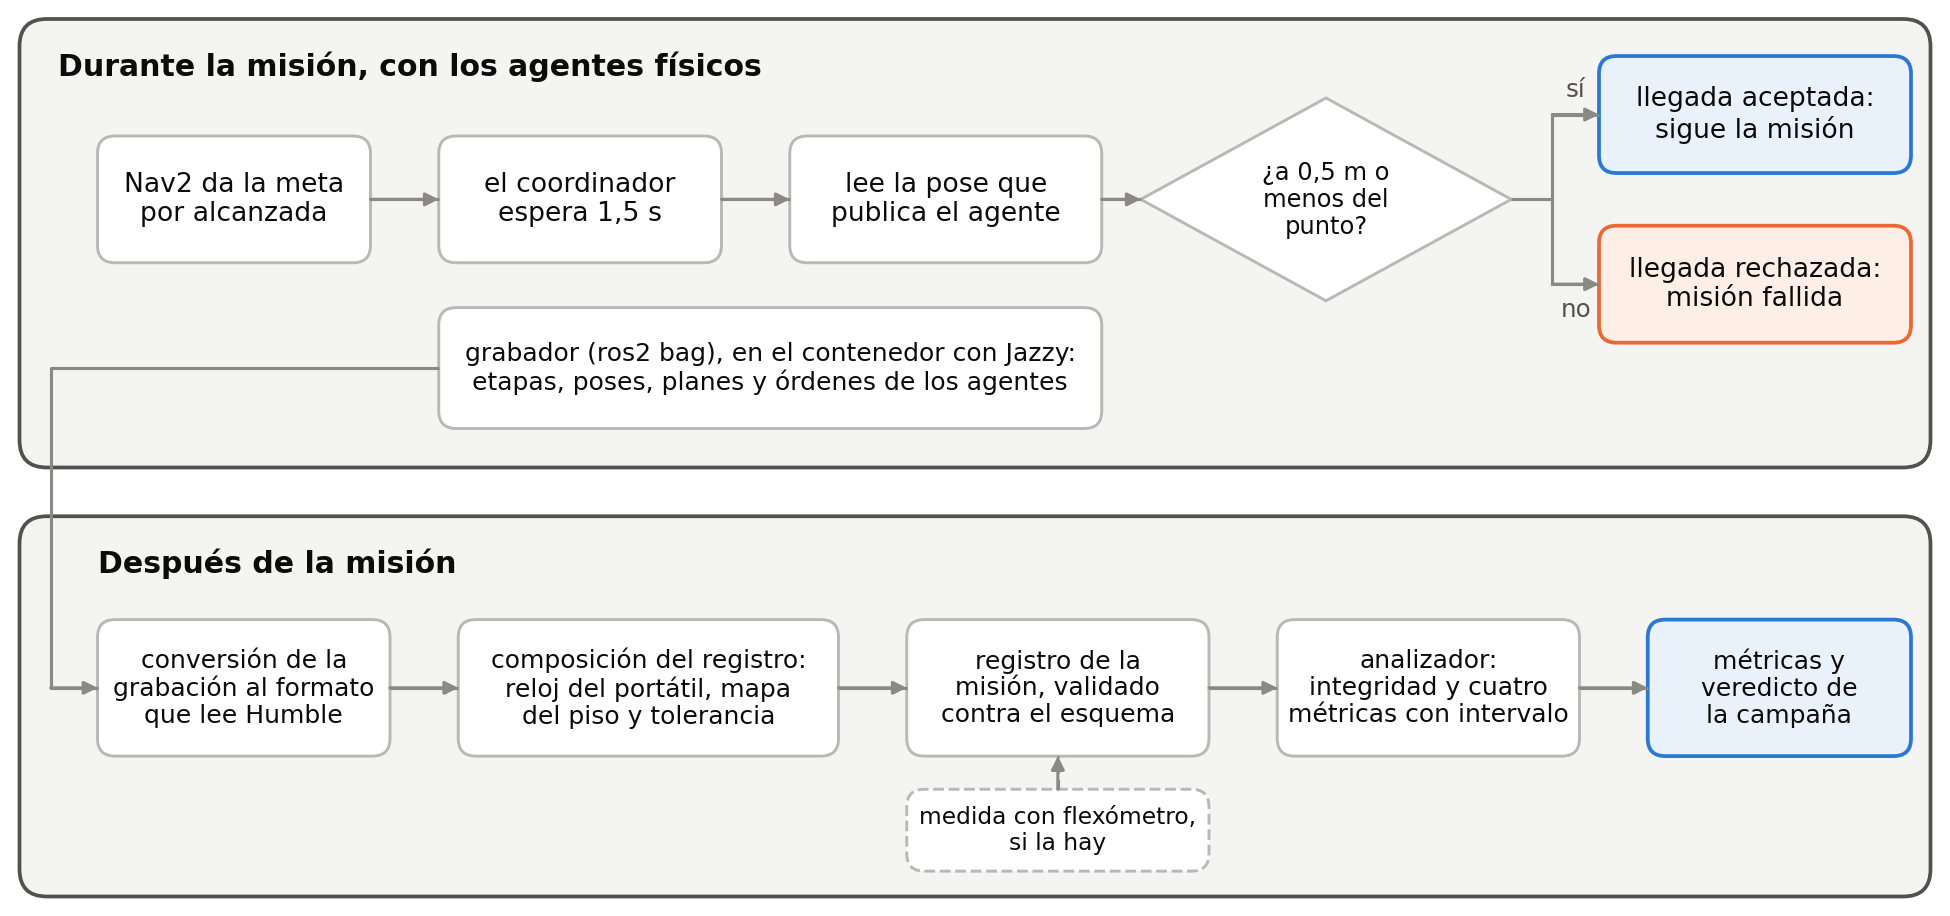
\includegraphics[width=0.7\textwidth]{imagenes/instrumentacion.png}
  \caption{Instrumentación de una misión: verificación de la llegada con los agentes físicos (arriba) y camino de la grabación hasta las métricas (abajo).}
  \label{fig:instrumentacion}
\end{figure}

% =====================================================================
\section{Cumplimiento de los objetivos específicos}
\label{sec:cumplimiento}

Un objetivo se considera cumplido cuando todos sus requisitos tienen verificada la prueba que los declara cumplidos (tabla~\ref{tab:cumplimiento}). Las siete restricciones del alcance también quedaron verificadas, con lo que la matriz cierra con treinta y seis de treinta y seis.

\begin{table}[H]
  \centering\footnotesize\setstretch{1.0}
  \caption{Cumplimiento de cada objetivo específico: cómo se cumplió, requisitos verificados y evidencia.}
  \label{tab:cumplimiento}
  \begin{tabular}{@{}>{\raggedright\arraybackslash}p{0.15\textwidth}>{\raggedright\arraybackslash}p{0.41\textwidth}>{\raggedright\arraybackslash}p{0.1\textwidth}>{\raggedright\arraybackslash}p{0.26\textwidth}@{}}
    \toprule
    \textbf{Objetivo} & \textbf{Cómo se cumplió} & \textbf{Requisitos} & \textbf{Evidencia} \\ \midrule
    1. Arquitectura funcional & Matriz de requisitos, escenarios en los edificios Gregorio y Catalayud, asignación por piso con un planificador comprobado en 930 combinaciones y contrato de interfaces & 10 de 10 & Relevo en simulación y con los agentes físicos (anexo A, videos 5 a 7) \\ \addlinespace
    2. Plataforma robótica & Dos agentes sobre AWS DeepRacer con locomoción, sensado, procesamiento y comunicación integrados & 6 de 6 & Seis pruebas de verificación superadas (anexo A, videos 1 a 4 y 7) \\ \addlinespace
    3. Interfaz móvil & Página web con selección de origen y destino, confirmación de cambio de piso y cancelación & 6 de 6 & Probada en un teléfono con los agentes físicos (anexo A, video 8) \\ \addlinespace
    4. Evaluación & Cuatro métricas con definición operativa, treinta misiones en simulación y nueve con los agentes físicos & 7 de 7 & Registros de cada misión (anexo B) y campañas (anexo A, videos 6 y 7) \\ \bottomrule
  \end{tabular}
\end{table}
